% =============================================================================
% Fallstudien zur Finanzwirtschaft
% Risikomodellierung und Risikoprognose mit GARCH-Modellen
%
% Aufbau: Einleitung, Daten, Methodik, Ergebnisse, Einordnung in die Literatur,
% Limitationen, Fazit sowie Anhang zur synthetischen Validierung.
% Die Literatur wird ausschliesslich in der Einleitung eingefuehrt, in der
% Methodik nur dort erneut zitiert, wo ein Verfahren begruendet wird, und in
% Abschnitt 5 nur noch gegen die eigenen Befunde gehalten.
%
% Alle Tabellen liegen als eigene Dateien in Abbildungen/ und werden von
% ../paper/tabellen.py aus den Ergebnis-CSVs erzeugt:
%     python paper/tabellen.py
% =============================================================================
\documentclass[12pt,a4paper]{article}

\usepackage[utf8]{inputenc}
\usepackage[T1]{fontenc}
\usepackage[ngerman]{babel}
% Times-Klon fuer Text und Mathematik (metrisch identisch zu Times New Roman);
% newtxmath stellt auch die AMS-Symbole bereit, amssymb entfaellt dadurch
\usepackage{amsmath}
\usepackage{newtxtext,newtxmath}
\usepackage{microtype}
\usepackage{booktabs}
\usepackage{graphicx}
\usepackage{xcolor}
\usepackage[normalem]{ulem}
% Aenderungsmarkierung: \neu{...} = neuer Text (rot), \alt{...} = zu streichender Text (rot, durchgestrichen)
\long\def\neu#1{\textcolor{red}{#1}}
\long\def\alt#1{\textcolor{red}{\sout{#1}}}
% Seitenraender: links 3,5 cm (Bindung), rechts 1,5 cm, oben 2,5 cm, unten 2 cm
\usepackage[a4paper,left=3.5cm,right=1.5cm,top=2.5cm,bottom=2cm]{geometry}
\usepackage{setspace}
\usepackage[hidelinks]{hyperref}
\usepackage{subcaption}
\captionsetup[table]{position=bottom,skip=6pt,justification=centering}
\usepackage{csquotes}
\usepackage[backend=biber,style=apa]{biblatex}
\DeclareLanguageMapping{ngerman}{ngerman-apa}
% APA verlangt "et al." statt der deutschen Abkuerzung "u. a."
\DefineBibliographyStrings{ngerman}{%
  andothers = {et\addabbrvspace al\adddot},
}
\addbibresource{literatur.bib}

\onehalfspacing
% Blocksatz ist LaTeX-Standard, Silbentrennung kommt aus babel/ngerman;
% die gelockerten Toleranzen vermeiden zu weite Wortabstaende in langen Zeilen
\tolerance=2000
\emergencystretch=1em
\setlength{\parindent}{0pt}
\setlength{\parskip}{0.6em}

% Gleitobjekte duerfen mehr einer Seite einnehmen, bevor LaTeX sie auf eine
% eigene Gleitseite schiebt; so bleibt Text neben Tabellen und Abbildungen
\renewcommand{\topfraction}{0.9}
\renewcommand{\bottomfraction}{0.8}
\renewcommand{\textfraction}{0.07}
\renewcommand{\floatpagefraction}{0.75}

\title{Risikobasierte Portfoliooptimierung mit GARCH-Modellen}
\author{}
\date{}

\begin{document}
\maketitle

\renewcommand{\abstractname}{Abstrakt}
\begin{abstract}
\iffalse
Diese Arbeit untersucht, ob risikobasierte Portfolioverfahren das naive 1/N-Portfolio schlagen und ob GARCH- und DCC-GARCH-Prognosen der Kovarianzmatrix gegenüber einer historischen Schätzung einen Mehrwert stiften.
Die Grundlage bilden tägliche Renditen von 27~US-Sektorindizes über gut 27~Jahre, die in zehn Trainingsfenstern und vier Prognosehorizonten und damit in 40~Konstellationen ausgewertet werden.
Bewertet wird getrennt nach statistischen und ökonomischen Kriterien.
Statistisch fällt das Ergebnis eindeutig aus, da DCC-GARCH die Kovarianzmatrix unter dem primären QLIKE-Kriterium in 37 und unter dem MSE in allen 40~Konstellationen besser prognostiziert als die historische Matrix.
Ökonomisch schlägt sich dieser Vorsprung allenfalls beim Minimum-Varianz-Portfolio nieder, während er bei Hierarchical Risk Parity und Equal Risk Contribution folgenlos bleibt.
Belastbar ist er jedoch auch dort nicht, da sämtliche Tests auf Sharpe-Differenzen insignifikant ausfallen.
Ausschlaggebend ist der Turnover, der beim Minimum-Varianz-Portfolio mit dynamischer Kovarianz um den Faktor~32 höher liegt und die dynamischen Varianten unter realen Handelskosten zusätzlich belasten würde.
Eine bessere Risikoprognose ist folglich nicht automatisch eine bessere Anlageentscheidung.
\neu{Code und Daten liegen im begleitenden Repository.}
\fi
\end{abstract}

% =============================================================================
\section{Einleitung}
\iffalse
Seit \textcite{markowitz1952} ist die Zusammenstellung eines Portfolios als Optimierungsproblem formuliert, bei dem die Gewichte gesucht werden, die bei gegebener erwarteter Rendite die Portfoliovarianz minimieren.
In der praktischen Anwendung erweist sich dieser Ansatz jedoch als fragil, da sowohl die Erwartungswerte als auch die Kovarianzmatrix aus historischen Daten geschätzt werden müssen.
Weil das Verfahren Anlagen mit zufällig überschätzter Rendite systematisch übergewichtet, verstärkt es Schätzfehler, statt sie auszumitteln.
\textcite{michaud1989} bezeichnet die Markowitz-Optimierung deshalb als Fehlermaximierung.

Von diesem Problem sind die beiden Eingangsgrößen unterschiedlich stark betroffen.
\textcite{broadie1993} zeigt in einer Simulationsstudie, dass Fehler in den geschätzten Erwartungswerten die Lage der effizienten Grenze deutlich stärker verzerren als Fehler in den geschätzten Varianzen und Kovarianzen.
Erwartete Renditen lassen sich aus Kursdaten nur mit großer Unsicherheit bestimmen, während Risikokennzahlen stabiler zu schätzen sind.
Wie gravierend die Folgen sind, zeigen \textcite{demiguel2009}, da in ihrem Vergleich über mehrere Datensätze keine der optimierten Strategien das naive, gleichgewichtete 1/N-Portfolio verlässlich schlagen konnte.
Der Aufwand einer Optimierung lohnt sich folglich nur, wenn ihr Gewinn den Verlust durch Schätzfehler übersteigt.

An dieser Stelle setzen risikobasierte Portfolioverfahren an, die vollständig auf Renditeprognosen verzichten und die Gewichte allein aus der Kovarianzmatrix bestimmen.
Untersucht werden hier das Minimum-Varianz-Portfolio, das Equal-Risk-Contribution-Portfolio sowie die Hierarchical Risk Parity (HRP) von \textcite{deprado2016}.
Die drei Verfahren unterscheiden sich vor allem darin, wie intensiv sie die geschätzte Kovarianzmatrix nutzen, weshalb deren Qualität unterschiedlich stark auf die Gewichte durchschlägt.
Gerade diese Abstufung macht sie zu einem geeigneten Prüffeld für die Frage, wie viel eine bessere Risikoprognose überhaupt wert sein kann.

Damit rückt die Kovarianzmatrix selbst in den Mittelpunkt, denn werden die Gewichte ausschließlich aus ihr abgeleitet, sollte eine bessere Schätzung auch zu besseren Portfolios führen.
Der übliche Stichprobenschätzer unterstellt jedoch konstante Varianzen und Korrelationen über das gesamte Schätzfenster.
Diese Annahme widerspricht der Beobachtung, dass ruhige und turbulente Phasen einander ablösen und große Kursausschläge weitere große Ausschläge nach sich ziehen.
\textcite{engle1982} hat diese Volatilitätscluster erstmals ökonometrisch erfasst, worauf \textcite{bollerslev1986} das heute übliche Generalized-Autoregressive-Conditional-Heteroskedasticity-Modell (GARCH) aufbaute.

Für ein Portfolio genügt es allerdings nicht, die Varianzen einzeln zu modellieren, da auch die Abhängigkeitsstruktur zwischen den Anlagen zeitvariabel ist.
Dass Korrelationen in Stressphasen ansteigen und die Diversifikation gerade dann versagt, wenn sie am dringendsten gebraucht wird, kann ein Modell mit konstanter Korrelation nicht abbilden.
\textcite{engle2002} überträgt die GARCH-Rekursion deshalb auf die Korrelationsmatrix selbst und erhält mit dem Dynamic-Conditional-Correlation-Modell (DCC) eine vollständig zeitvariable Kovarianzprognose.
Dass diese Erweiterung für die Allokation relevant ist, legen \textcite{ardia2017} nahe, die eine Fehlspezifikation der Kovarianzmatrix als spürbare Verzerrung der Gewichte risikobasierter Portfolios ausweisen.

Ob eine statistisch bessere Prognose auch zu einer besseren Anlageentscheidung führt, ist damit jedoch nicht beantwortet.
\textcite{engle2006} weisen darauf hin, dass die Sharpe Ratio als Kriterium für die Auswahl eines Kovarianzschätzers irreführend sein kann, da sie von den realisierten Renditen dominiert wird, auf die die Kovarianzmatrix nur mittelbar wirkt.
Als Alternative bietet \textcite{patton2011} Verlustfunktionen an, deren Rangfolge auch bei einem verrauschten Proxy der wahren Varianz erhalten bleibt, während \textcite{laurent2013} dieses Konzept auf vollständige Kovarianzmatrizen übertragen.
Wie weit beide Kriterien auseinanderfallen können, zeigen \textcite{moura2020} für hochdimensionale bedingte Kovarianzmatrizen, wo die statistisch beste Spezifikation nicht die ökonomisch beste ist.

Die Verbindung beider Themenfelder, risikobasierter Allokation einschließlich neuerer Verfahren wie HRP auf der einen und multivariater GARCH-Prognosen auf der anderen Seite, ist bislang nur vereinzelt untersucht worden.
Vor diesem Hintergrund verfolgt diese Arbeit zwei Fragen.
Erstens wird geprüft, ob Minimum-Varianz-, Equal-Risk-Contribution- und Hierarchical-Risk-Parity-Portfolios eine höhere risikoadjustierte Out-of-Sample-Performance erzielen als das naive 1/N-Portfolio.
Zweitens wird untersucht, ob GARCH- und DCC-GARCH-basierte Risiko- und Kovarianzprognosen die Ergebnisse gegenüber einer historischen Schätzung verbessern.
Beide Fragen werden getrennt nach statistischen und ökonomischen Kriterien beantwortet, da sich gerade in der Differenz zwischen beiden der zentrale Befund dieser Arbeit zeigt.

Die empirische Grundlage bilden tägliche Renditen von 27~US-Sektorindizes über gut 27~Jahre.
Zehn Trainingsfenster und vier Prognosehorizonte ergeben 40~Konstellationen, in denen jede der drei Kovarianzschätzungen mit \neu{jedem der drei risikobasierten Verfahren, jeweils gegen das 1/N-Portfolio,}\alt{jedem der vier Allokationsverfahren} bewertet wird.
Als Kriterien dienen statistisch QLIKE-Verlust und Kovarianz-MSE, ökonomisch Sharpe Ratio, realisierte Volatilität und Turnover.
Ergänzend prüfen drei simulierte Datensätze mit bekanntem datengenerierendem Prozess, ob die Modelle das leisten, wofür sie konstruiert sind.

Diesem Vorgehen folgt auch der weitere Aufbau der Arbeit.
Der \hyperref[sec:daten]{folgende Abschnitt} beschreibt die Datengrundlage, während der \hyperref[sec:methodik]{\ref*{sec:methodik}.~Abschnitt} das Untersuchungsdesign darlegt.
Im \hyperref[sec:ergebnisse]{\ref*{sec:ergebnisse}.~Abschnitt} werden die Ergebnisse zunächst zur Prognosequalität und anschließend zur Portfolioperformance berichtet, bevor ihre Stabilität über verschiedene Zeiträume und Anlageuniversen untersucht wird.
Anschließend ordnet der \hyperref[sec:literatur]{\ref*{sec:literatur}.~Abschnitt} die Befunde in die Literatur ein und der \hyperref[sec:limitationen]{\ref*{sec:limitationen}.~Abschnitt} diskutiert die Grenzen der Untersuchung.
Am Ende werden die zentralen Erkenntnisse zusammengefasst.

% =============================================================================
\fi
\section{Daten}\label{sec:daten}
\iffalse
In diesem Abschnitt wird die Datengrundlage der empirischen Untersuchung beschrieben.
Dabei wird zwischen den empirischen Sektordaten und den simulierten Datensätzen unterschieden.
\fi

\subsection{Sektorindizes}
\iffalse
Verwendet werden tägliche Kurse US-amerikanischer Sektorindizes, die über Datastream bezogen wurden.
Als Sektorabgrenzung dienen die Business Groups der Refinitiv Business Classification (TRBC), wobei für die Vereinigten Staaten nur Daten für 28 der insgesamt 32~Business Groups verfügbar sind.
Eine davon zeigt an rund zwei Dritteln ihrer Datenpunkte keine Kursbewegung und wird als inaktive Reihe verworfen, sodass 27~Sektoren in die Analyse eingehen.
Der Beobachtungszeitraum reicht vom 02.04.1999 bis zum 09.06.2026 und umfasst 7.087 Handelstage, wobei nur für 16~Sektorindizes Daten über die gesamte Historie vorliegen, während die übrigen Datenreihen erst zu späteren Zeitpunkten starten.

Die Querschnittsverteilung der Sektorrenditen ist in \hyperref[tab:daten_deskriptiv]{Tabelle~\ref*{tab:daten_deskriptiv}} dargestellt.
Auffällig ist dabei die durchschnittliche paarweise Korrelation von 0,562, die aufgrund der Begrenzung auf den US-Aktienmarkt erwartungsgemäß hoch ausfällt und die Diversifikationsmöglichkeiten innerhalb des Universums von vornherein einschränkt.
% [Vorschlag 2.1] Halbsatz zu 260 vs. 252 Handelstagen/Jahr auf Wunsch wieder
% entfernt (zu kleinteilig, praeferenzabhaengig ob relevant fuer den Betreuer).
%\neu{Mit 7.087 Handelstagen über 27,2 Jahre entfallen im Mittel rund 260 statt der üblichen 252 Tage auf ein Jahr, da Datastream Feiertage mit dem Kurs des Vortages auffüllt und diese damit als Handelstage mit Nullrendite in der Reihe erscheinen; auf eine Bereinigung wurde verzichtet, da sie die Schätzungen nur geringfügig verändert. Auf die 252er-Annualisierung sowie auf leicht gedrückte Varianz- und Korrelationsschätzungen wird in den \hyperref[sec:limitationen]{Limitationen} zurückgekommen.}
\fi

% automatisch erzeugt von paper/tabellen.py -- nicht von Hand editieren
\begin{table}[htbp]
  \centering
  \footnotesize
  \begin{tabular}{lrrrrr}
    \toprule
    Kennzahl & Min. & 25\,\% & Median & 75\,\% & Max. \\
    \midrule
    Beobachtungen & 1351 & 1877 & 7087 & 7087 & 7087 \\
    Rendite p.a. (\%) & -5,34 & 4,70 & 6,02 & 8,97 & 20,27 \\
    Volatilität p.a. (\%) & 15,06 & 19,73 & 22,41 & 26,32 & 49,20 \\
    \bottomrule
  \end{tabular}
  \caption{Deskriptive Statistik der TRBC-Sektorrenditen}
  \label{tab:daten_deskriptiv}
  \begin{minipage}{\linewidth}\vspace{0.4em}\centering\footnotesize
  Tägliche logarithmierte Renditen von 27 TRBC-Sektorindizes, 02.04.1999 bis 09.06.2026; durchschnittliche paarweise Korrelation 0,562.
  \end{minipage}
\end{table}


\subsection{Risikofreier Zins}
\iffalse
Als risikofreier Zinssatz dient die Fed Funds Rate, die wie auch die Sektorindizes über Datastream bezogen wird.
\neu{Bezogen wird sie als täglicher Total-Return-Index, sodass die tägliche risikofreie Rendite direkt als dessen prozentuale Veränderung berechnet wird, ohne eine annualisierte Rate erst auf Tagesbasis umrechnen zu müssen.}
Sie fließt nicht in die Optimierung der einzelnen Portfolios ein, sondern wird ausschließlich für die Berechnung der Sharpe Ratio verwendet.
\fi

\subsection{Synthetische Datensätze}
\iffalse
Hinzu kommen drei künstlich erzeugte Datensätze, die ausschließlich der Validierung der Implementierung dienen.
Simuliert werden ein Prozess mit konstanter Kovarianzmatrix sowie je ein CCC- und ein DCC-GARCH-Prozess, sodass für jeden der drei Kovarianzschätzer ein Datensatz vorliegt, auf dem er korrekt spezifiziert ist.
Auf diese Weise lässt sich prüfen, ob die Modelle genau die Struktur erkennen, für die sie konstruiert sind, was an echten Daten wegen des unbekannten datengenerierenden Prozesses nicht möglich ist.
Die Parametrisierung ist im \hyperref[sec:anhang_synth]{Anhang~\ref*{sec:anhang_synth}} dokumentiert.

% =============================================================================
\fi
\section{Methodik}\label{sec:methodik}
\iffalse
In diesem Abschnitt wird das Untersuchungsvorgehen vorgestellt.
Dabei wird auf die Schätzung der Kovarianzmatrix, die Portfoliooptimierung und die Bewertungskriterien eingegangen.
\fi

\subsection{Rolling Window}\label{subsec:rollfenster}
\iffalse
Um für mögliche Strukturbrüche in den Daten zu kontrollieren und zugleich einer realistischen Anwendung nahe zu kommen, wird ein Rolling-Window-Ansatz gewählt.
Die Kovarianzmatrix wird dabei auf einem Trainingsfenster der Länge $T$ geschätzt, wobei alle Modellparameter an jedem Termin neu bestimmt werden, daraus werden die Portfoliogewichte bestimmt und diese über den Prognosehorizont von $h$ Handelstagen gehalten, bevor das Fenster um $h$ Tage weiterrückt.
Variiert werden beide Größen, wobei das Trainingsfenster zwischen einem und zehn Jahren liegt und der Prognosehorizont 1, 5, 10 oder 21 Handelstage beträgt.
Der Vergleich der daraus resultierenden 40~Kombinationen zeigt zum einen, ob die Befunde robust gegenüber der Wahl von Trainings- und Prognosefenster sind, und zum anderen, bei welcher Fensterlänge sich Schätzfehler aus zu wenigen Beobachtungen und Fehlspezifikation aus sich ändernden Parametern am besten ausgleichen.
Als Basisfall werden durchgängig $T = 1008$ (vier Jahre) und $h = 1$ berichtet und von da ausgehend die Robustheit der Ergebnisse überprüft.

Je Zeitfenster werden dabei nur Sektoren berücksichtigt, die an mindestens 90\,\% der Handelstage verfügbar sind, um so eine ausreichende Datenbasis für die Schätzung zu gewährleisten und zugleich nicht ganze Anlagen wegen einzelner fehlender Datenpunkte auszuschließen.
Das investierbare Universum wird somit in jedem Fenster neu bestimmt und variiert sowohl über die Zeit als auch über die Fensterlänge.

Ein Nachteil des Untersuchungsdesigns ist jedoch, dass ein längeres Trainingsfenster den Out-of-Sample-Zeitraum verkürzt.
So beginnt dieser bei einem Jahr Trainingsdaten bereits im März~2000, bei zehn Jahren dagegen erst im November~2008.
Der lange Lauf \neu{setzt damit erst nach dem Kurssturz vom Herbst 2008 ein und erfasst}\alt{schließt damit den Einbruch der Finanzkrise aus und deckt} im Wesentlichen nur die anschließende Erholung ab.
Diese Unterschiede führen dazu, dass die Ergebnisse durch die jeweils abgedeckten Marktphasen beeinflusst werden, wodurch die Vergleichbarkeit eingeschränkt wird.
Sämtliche Vergleiche über Trainingsfenster und Prognosehorizonte werden daher auf dem gemeinsamen Bewertungszeitraum ab dem 01.01.2010 gerechnet, sodass alle Testzeiträume rund 4.280 Handelstage umfassen und alle Ergebnisse über die gleichen Marktphasen bestimmt werden.
Der Basisfall wird zusätzlich zuerst über seine volle verfügbare Historie ab Februar~2003 berichtet, da sich die Frage der Vergleichbarkeit dort nicht stellt.
Wie weit beide Rechnungen auseinanderliegen, zeigt \hyperref[sec:anhang_strukturbruch]{Anhang~\ref*{sec:anhang_strukturbruch}}.
\fi

\subsection{Kovarianzschätzer}\label{subsec:kovarianz}
\iffalse
Verglichen werden drei Schätzer der bedingten Kovarianzmatrix, die eine aufsteigende Leiter an Dynamik abbilden.
Den Ausgangspunkt bildet der statische historische Schätzer, der zunächst um eine zeitvariable Varianz im GARCH-Modell und anschließend um eine dynamische Korrelation im DCC-GARCH-Modell erweitert wird.
Da jeder Schritt genau eine Annahme aufhebt, lässt sich der Beitrag der jeweiligen Komponente isoliert bewerten.
\fi

\paragraph{Historische Kovarianzmatrix:}
\iffalse
Verwendet wird zunächst die Stichprobenkovarianz der Trainingsrenditen, in der die Annahme konstanter Varianzen und Korrelationen über das gesamte Fenster unverändert erhalten bleibt.

Der Vorteil dieses Schätzers liegt in seiner Einfachheit, da er keine Parameterschätzung im engeren Sinn benötigt und deshalb weder von Konvergenzproblemen noch von einer Fehlspezifikation der Dynamik betroffen sein kann.
Dem steht seine Trägheit gegenüber, weil ein Volatilitätsschock nur mit einem geringen Gewicht in die Schätzung eingeht und erst nach $T$ Handelstagen wieder aus ihr verschwindet.
Aus diesen Gründen dient die historische Matrix in dieser Arbeit als statischer Referenzpunkt, gegen den der Mehrwert der beiden dynamischen Modelle gemessen wird.
\fi

\paragraph{Generalized Autoregressive Conditional Heteroskedasticity (GARCH):}
\iffalse
Das GARCH-Modell wurde im Jahr \citeyear{bollerslev1986} von \citeauthor{bollerslev1986} vorgestellt und verallgemeinert das ARCH-Modell, mit dem \textcite{engle1982} die zeitvariable Varianz von Finanzzeitreihen erstmals ökonometrisch erfasst hatte.
Beide Modelle greifen die Beobachtung auf, dass große Kursausschläge gehäuft auftreten und weitere große Ausschläge nach sich ziehen, was der historische Schätzer per Konstruktion ignoriert.
Der Grundgedanke besteht darin, die Varianz nicht als Konstante, sondern als bedingte Größe zu behandeln, die aus der Information bis zur Vorperiode fortgeschrieben wird.

Ein GARCH(1,1) beschreibt die Rendite als Summe aus einem konstanten Mittelwert und einem Störterm, dessen Varianz einer eigenen Rekursion folgt.
% [Vorschlag 3.6] Satz zur Schaetzung von mu (arch-Paket, MLE statt
% Stichprobenmittel) auf Wunsch wieder entfernt -- zu implementierungsnah.
%\neu{Der Mittelwert $\mu$ wird dabei nicht als Stichprobenmittel vorgegeben, sondern zusammen mit $\omega$, $\alpha$ und $\beta$ durch dieselbe Maximum-Likelihood-Schätzung des Pakets \texttt{arch} bestimmt.}

\begin{align}
	\label{eq:garch-1}
	r_t &= \mu + \varepsilon_t \\
	\label{eq:garch-2}
	\varepsilon_t &= \sqrt{h_t}\,z_t, \qquad z_t \sim \mathcal{N}(0,1) \\
	\label{eq:garch-3}
	h_t &= \omega + \alpha\,\varepsilon_{t-1}^2 + \beta\,h_{t-1}
\end{align}

Die bedingte Varianz $h_t$ setzt sich damit aus drei Bestandteilen zusammen (\hyperref[eq:garch-3]{Gleichung~\ref*{eq:garch-3}}).
Die Konstante $\omega$ verankert das langfristige Varianzniveau, während $\alpha$ steuert, wie stark ein neuer Schock die Varianz bewegt, und $\beta$ misst, wie lange dieser Einfluss anhält.
Damit die unbedingte Varianz existiert und der Prozess stationär bleibt, müssen $\omega > 0$, $\alpha, \beta \geq 0$ sowie $\alpha + \beta < 1$ gelten \parencite{bollerslev1986}.

Da die Portfoliogewichte nicht nur für den Folgetag, sondern für die kommenden $h$ Handelstage gelten, wird die Rekursion über den Horizont fortgeschrieben und anschließend gemittelt.
Weil der erwartete quadrierte Schock der bedingten Varianz entspricht, vereinfacht sich die Fortschreibung ab dem zweiten Schritt zu einer Konvergenz gegen die unbedingte Varianz.

\begin{align}
	\label{eq:garch-fc-1}
	\mathrm{E}_t[h_{t+k}] &= \omega + (\alpha + \beta)\,\mathrm{E}_t[h_{t+k-1}], \qquad k \geq 2 \\
	\label{eq:garch-fc-2}
	\bar{h}_{t,h} &= \frac{1}{h}\sum_{k=1}^{h} \mathrm{E}_t[h_{t+k}]
\end{align}

Die horizontgemittelte Varianzprognose $\bar{h}_{t,h}$ aus \hyperref[eq:garch-fc-2]{Gleichung~\ref*{eq:garch-fc-2}} geht als Diagonalelement in die Kovarianzmatrix ein.

Für ein Portfolio genügt die Modellierung der einzelnen Varianzen allerdings nicht, da für die Gewichte die vollständige Kovarianzmatrix benötigt wird.
Die Umsetzung folgt deshalb dem Constant-Conditional-Correlation-Ansatz (CCC) von \textcite{bollerslev1990}, bei dem für jeden Sektor ein eigenes GARCH(1,1) geschätzt, die Korrelationsmatrix dagegen konstant gehalten wird:

\begin{equation}
	\Sigma_t = D_t\,R\,D_t, \qquad D_t = \operatorname{diag}\left(\sqrt{\bar{h}_{1}}, \dots, \sqrt{\bar{h}_{N}}\right)
	\label{eq:ccc}
\end{equation}

Die Diagonalmatrix $D_t$ enthält die prognostizierten Standardabweichungen der $N$ Sektoren, während $R$ als Stichprobenkorrelation der standardisierten Residuen $z_t$ aus \hyperref[eq:garch-2]{Gleichung~\ref*{eq:garch-2}} geschätzt wird.
\neu{Dabei bezeichnet $\bar{h}_i$ die horizontgemittelte Varianzprognose $\bar{h}_{t,h}$ aus \hyperref[eq:garch-fc-2]{Gleichung~\ref*{eq:garch-fc-2}} für Sektor $i$, wobei der Zeit- und Horizontindex der Übersichtlichkeit halber unterdrückt wird.}
Diese werden statt der Rohrenditen verwendet, da in ihnen die Volatilitätscluster bereits herausgefiltert sind und Tage hoher Volatilität die Korrelationsschätzung sonst verzerren würden.
Gegenüber der historischen Matrix ändert sich damit ausschließlich die Behandlung der Varianzen, wodurch der Vergleich beider Schätzer den Beitrag der dynamischen Volatilität isoliert.
\fi

\paragraph{Dynamic Conditional Correlation (DCC-GARCH):}
\iffalse
Da das GARCH-Modell weiterhin von einer konstanten Korrelation ausgeht, die in der Realität nur selten vorliegt, entwickelte \textcite{engle2002} mit dem DCC-GARCH-Modell eine Erweiterung, die auch diese Restriktion aufhebt.
\citeauthor{engle2002} überträgt dafür die Rekursion aus \hyperref[eq:garch-3]{Gleichung~\ref*{eq:garch-3}} auf die Korrelation selbst und erhält so eine vollständig zeitvariable Kovarianzprognose.

Modelliert wird dabei zunächst eine Hilfsmatrix $Q_t$, die anschließend zu einer gültigen Korrelationsmatrix normiert wird.

\begin{align}
	\label{eq:dcc-1}
	Q_t &= (1 - a - b)\,\bar{Q} + a\,z_{t-1}z_{t-1}' + b\,Q_{t-1} \\
	\label{eq:dcc-2}
	R_t &= \operatorname{diag}(Q_t)^{-1/2}\,Q_t\,\operatorname{diag}(Q_t)^{-1/2} \\
	\label{eq:dcc-3}
	\Sigma_t &= D_t\,R_t\,D_t
\end{align}

Der Aufbau von \hyperref[eq:dcc-1]{Gleichung~\ref*{eq:dcc-1}} entspricht dem der GARCH-Rekursion, wobei $\bar{Q}$ die Rolle des langfristigen Niveaus übernimmt und auf die Stichprobenkorrelation der standardisierten Residuen gesetzt wird.
Wie stark die Korrelationen auf neue gemeinsame Schocks reagieren, misst der Parameter $a$, während $b$ deren Persistenz angibt.
Analog zum univariaten Fall müssen dafür $a, b \geq 0$ und $a + b < 1$ gelten.
Da $Q_t$ auf der Diagonale keine Einsen aufweisen muss, ist die Normierung in \hyperref[eq:dcc-2]{Gleichung~\ref*{eq:dcc-2}} nötig, um eine Korrelationsmatrix zu erhalten.
Aus dieser und den prognostizierten Standardabweichungen ergibt sich die Kovarianzmatrix schließlich nach \hyperref[eq:dcc-3]{Gleichung~\ref*{eq:dcc-3}}.

Geschätzt wird das Modell in zwei Schritten, indem zuerst die univariaten GARCH-Modelle und anschließend die beiden Parameter $a$ und $b$ per Maximum-Likelihood auf den standardisierten Residuen bestimmt werden.
Für $h > 1$ wird die Korrelationsprognose gemäß \textcite{engle2001} auf $\bar{Q}$ zurückgeführt und über den Horizont gemittelt, damit sie zur ebenfalls horizontgemittelten Varianzprognose passt.

Da GARCH- und DCC-Schätzer dieselben Varianzprognosen und dieselben standardisierten Residuen verwenden, isoliert ihr Vergleich exakt den Beitrag der dynamischen Korrelation.
Die drei Schätzer bilden somit die eingangs beschriebene Leiter, deren Stufen sich um jeweils genau eine Annahme unterscheiden.
\fi

\subsection{Portfoliomodelle}\label{subsec:portfolios}
\iffalse
Allen drei risikobasierten Allokationsverfahren ist gemeinsam, dass in ihre Gewichte ausschließlich die zweiten Momente eingehen und keine Renditeprognose benötigt wird.
Das als Vergleichsmaßstab herangezogene 1/N-Portfolio kommt sogar ohne diese aus.
Damit entfällt die Fehlerquelle, die nach \textcite{broadie1993} die Lage der effizienten Grenze am stärksten verzerrt.
Berücksichtigt werden Verfahren mit unterschiedlichen Zielen, die die geschätzte Kovarianzmatrix verschieden intensiv nutzen und deshalb auch verschieden empfindlich auf deren Fehler reagieren.
\fi

\paragraph{Minimum-Varianz-Portfolio (MVP)}
\iffalse
Das Minimum-Varianz-Portfolio bildet nach dem Ansatz von \textcite{markowitz1952} das Portfolio, das ohne Berücksichtigung der erwarteten Renditen die geringste Volatilität aufweist.
Daraus ergibt sich die folgende Zielfunktion:

\begin{equation}
	\min_{w}\ w'\Sigma w \qquad \text{unter} \qquad \mathbf{1}'w = 1, \quad w \geq 0
	\label{eq:mvp}
\end{equation}

Der Vektor $w$ enthält die Portfoliogewichte und $\Sigma$ die prognostizierte Kovarianzmatrix, während die Budgetrestriktion $\mathbf{1}'w = 1$ die Vollinvestition sicherstellt.
Zusätzlich wird mit $w \geq 0$ ein Leerverkaufsverbot gesetzt.
Nach \textcite{behr2008} überzeugt das MVP besonders in volatilen Marktphasen.

Zugleich ist es das anfälligste Verfahren, da die Minimierung gezielt die Richtungen kleinster geschätzter Varianz aufsucht, in denen die Schätzfehler relativ am größten sind.
Fehler werden dadurch nicht ausgemittelt, sondern verstärkt, weshalb \textcite{lee2011} auf die typischerweise stark konzentrierten MVP-Lösungen hinweist.
\fi

\paragraph{Equal Risk Contribution (ERC)}
\iffalse
Das Equal-Risk-Contribution-Portfolio verfolgt nach \textcite{maillard2010} das Ziel, das Gesamtrisiko nicht zu minimieren, sondern gleichmäßig auf die Anlagen zu verteilen.
Grundlage ist die Zerlegung der Portfoliovolatilität in die Risikobeiträge der einzelnen Anlagen, die sich in der Summe genau zur Gesamtvolatilität ergänzen.

\begin{align}
	\label{eq:erc-1}
	\mathrm{RC}_i &= \frac{w_i\,(\Sigma w)_i}{\sqrt{w'\Sigma w}} \\
	\label{eq:erc-2}
	\mathrm{RC}_i &= \mathrm{RC}_j \qquad \text{für alle } i, j
\end{align}

Der Risikobeitrag $\mathrm{RC}_i$ aus \hyperref[eq:erc-1]{Gleichung~\ref*{eq:erc-1}} ist das Produkt aus dem Gewicht der Anlage und ihrem Grenzrisikobeitrag, wobei die Gewichte so bestimmt werden, dass alle Beiträge übereinstimmen (\hyperref[eq:erc-2]{Gleichung~\ref*{eq:erc-2}}).
% [Vorschlag 3.4] Satz zum Loesungsweg (riskfolio-Risk-Parity-Optimierung) auf
% Wunsch wieder entfernt -- zu implementierungsnah.
%\neu{Gelöst wird dieses Gleichungssystem numerisch über die Risk-Parity-Optimierung des Pakets \texttt{riskfolio} mit gleichen Zielbeiträgen für alle Anlagen.}
Anders als das MVP nutzt ERC die Kovarianzmatrix somit nur über das Produkt $\Sigma w$ und nicht über ihre Inverse, weshalb Schätzfehler weniger stark durchschlagen und ein robusteres Portfolio entsteht.

Das Ergebnis liegt konstruktionsbedingt zwischen dem MVP und dem gleichgewichteten Portfolio und ist in der Regel deutlich besser diversifiziert.
Dennoch schlägt ERC das naive Portfolio nach \textcite{chaves2011} nicht durchgängig.
\fi

\paragraph{Hierarchical Risk Parity (HRP)}
\iffalse
Hierarchical Risk Parity wurde von \textcite{deprado2016} mit dem Ziel entwickelt, die Matrixinversion des MVP durch eine hierarchische Struktur zu ersetzen und das Verfahren dadurch robuster gegenüber schlecht konditionierten Kovarianzmatrizen zu machen.
Der Algorithmus läuft in drei Schritten ab, von denen der erste die Korrelationen in eine Distanz überführt.

\begin{equation}
	d_{ij} = \sqrt{0{,}5\,(1 - \rho_{ij})}
	\label{eq:hrp}
\end{equation}

Zwei Sektoren stehen sich nach \hyperref[eq:hrp]{Gleichung~\ref*{eq:hrp}} umso näher, je höher ihre Korrelation $\rho_{ij}$ ausfällt.
Auf Basis dieser Distanz werden die Sektoren im zweiten Schritt zu einem Binärbaum geclustert und die Kovarianzmatrix quasi-diagonal geordnet, sodass ähnliche Anlagen nebeneinander stehen.
\neu{Geclustert wird dabei wie bei \textcite{deprado2016} mit Single Linkage, während Ward- oder Average-Linkage andere Bäume liefern würden.}
Im dritten Schritt wird das Kapital durch rekursive Bisektion verteilt, wobei die geordnete Liste wiederholt halbiert und das Gewicht zwischen beiden Hälften invers zu deren Varianz aufgeteilt wird.

Entscheidend ist, dass HRP die Kovarianzmatrix nie invertiert und von ihr nur die Ordnungsinformation sowie die Varianzen der Teilcluster nutzt.
Das Verfahren ist dadurch robuster als das MVP, verwertet aber im Umkehrschluss eine bessere Schätzung auch nur eingeschränkt.
\textcite{deprado2016} und \textcite{sen2022} berichten entsprechend stabilere Gewichte und eine konkurrenzfähige risikoadjustierte Rendite.
\fi

\paragraph{Benchmark}
\iffalse
Als Vergleichsmaßstab dient das gleichgewichtete 1/N-Portfolio, das jeder im Fenster verfügbaren Anlage denselben Anteil zuweist.
Es benötigt keine Schätzung der zweiten Momente und ist damit als einziges der vier Verfahren immun gegen Schätzfehler.

Das naive Portfolio bildet den relevanten Maßstab für die erste Forschungsfrage, da ein Optimierungsverfahren seinen Aufwand nur rechtfertigt, wenn dessen Gewinn den Verlust durch Schätzfehler übersteigt.
Wie hoch dieser Maßstab liegt, zeigt der Vergleich von \textcite{demiguel2009}, in dem keine der optimierten Strategien das gleichgewichtete Portfolio verlässlich schlagen konnte.
\fi

\subsection{Bewertungskriterien}\label{subsec:kriterien}
Die Bewertung trennt zwischen der Prognosequalität der Kovarianzmatrix und der ökonomischen Performance der daraus abgeleiteten Portfolios.

\paragraph{Statistische Verlustmaße}
Die Prognosequalität wird über zwei Verlustmaße gemessen, den multivariaten Quasi-Likelihood-Verlust (QLIKE), oder auch Stein-Loss genannt \parencite{laurent2013}, und den Mean Squared Error (MSE) der Kovarianzmatrix.
Da die wahre bedingte Kovarianzmatrix der Testperiode nicht beobachtbar ist, wird die Prognose bei beiden gegen denselben realisierten Proxy gemessen.

\begin{align}
	\label{eq:proxy}
	S &= \frac{1}{h}\sum_{t=1}^{h} r_t\,r_t' \\
	\label{eq:qlike}
	\mathrm{QLIKE}(\Sigma, S) &= \ln|\Sigma| + \operatorname{tr}(\Sigma^{-1} S) \\
	\label{eq:mse}
	\mathrm{MSE}(\Sigma, S) &= \frac{1}{N^2}\sum_{i,j}\left(\Sigma_{ij} - S_{ij}\right)^2
\end{align}

Dabei ist $\Sigma$ die prognostizierte und $S$ die realisierte Kovarianzmatrix, $r_t$ der Vektor der logarithmierten Tagesrenditen und $N$ die Anzahl der zur Verfügung stehenden Sektorindizes im jeweiligen Zeitfenster.
Beide Verluste werden je Rebalancierungsfenster berechnet und anschließend über die Fenster gemittelt, wobei niedrigere Werte eine bessere Prognose bedeuten.

Die beiden Maße unterscheiden sich darin, wie sie Fehler in beide Richtungen gewichten.
Der QLIKE-Verlust aus \hyperref[eq:qlike]{Gleichung~\ref*{eq:qlike}} bestraft eine Unterschätzung des Risikos stärker als eine Überschätzung, während der MSE aus \hyperref[eq:mse]{Gleichung~\ref*{eq:mse}} Über- und Unterschätzungen gleichgewichtet.
Aus ökonomischer Sicht wiegt eine Unterschätzung des Risikos schwerer als eine Überschätzung, weshalb die Asymmetrie des QLIKE-Verlusts hier erwünscht ist.

Diese beiden Maße werden verwendet, da sie sich in anderen Studien als robust gegenüber verrauschten Proxys erwiesen haben.
Dies ist insbesondere relevant, da der Proxy für $h=1$ allein aus dem äußeren Produkt eines einzigen Renditevektors besteht und somit stark verrauscht ist.
So konnten \textcite{patton2011} und \textcite{laurent2013} zeigen, dass beide Metriken Kovarianzmatrizen unabhängig von der Genauigkeit des Proxys robust ordnen.
Folglich ist der absolute Wert der Metriken zwar nur eingeschränkt interpretierbar, jedoch ist die Rangfolge robust, weshalb Qualitätsunterschiede zwischen den Schätzern erkannt werden können.
Da zusätzlich die Länge des Trainingsfensters die Zahl der investierbaren Anlagen und damit die Dimension der Kovarianzmatrix beeinflusst, sind Vergleiche zwischen den unterschiedlichen Trainingsfenstern ebenfalls mit Vorsicht zu interpretieren.
Aussagekräftig ist daher in erster Linie die Differenz zwischen den Schätzern innerhalb einer Spezifikation.

Da der QLIKE-Verlust ökonomisch besser motiviert ist, wird dieser als primäre Vergleichsmetrik verwendet, während der MSE als weitere Metrik zur Überprüfung der Robustheit dient.

\paragraph{Ökonomische Kennzahlen}
Als ökonomische Kennzahlen werden die annualisierte Rendite, die realisierte Volatilität, die Sharpe Ratio und der Turnover berichtet.
Die folgenden Kennzahlen beruhen auf der Tagesrendite der verschiedenen Portfolios $r_{p,t}$.

\begin{align}
	\label{eq:annrendite}
	R_{\mathrm{ann}} &= \left(\prod_{t=1}^{n}\left(1 + r_{p,t}\right)\right)^{\frac{252}{n}} - 1 \\
	\label{eq:annvola}
	\sigma_{\mathrm{ann}} &= \sqrt{252}\;\operatorname{sd}\left(r_{p,t}\right) \\
	\label{eq:sharpe}
	\text{Sharpe Ratio} &=\frac{252\;\overline{\left(r_{p,t} - r_{f,t}\right)}}{\sqrt{252}\;\operatorname{sd}\left(r_{p,t} - r_{f,t}\right)}
\end{align}

Die annualisierte Rendite aus \hyperref[eq:annrendite]{Gleichung~\ref*{eq:annrendite}} ist die geometrische Wachstumsrate über die $n$ Handelstage des Bewertungszeitraums, während die realisierte Volatilität als annualisierte Standardabweichung derselben Reihe berechnet wird.
Bei der Sharpe Ratio beruhen Zähler und Nenner auf der Überschussrendite gegenüber der Fed Funds Rate.

Neben diesen Metriken wird auch der Turnover beachtet, der angibt, welcher Anteil des Portfolios je Rebalancierung umgeschichtet wird.

\begin{equation}
	\mathrm{Turnover}_k = \sum_{i=1}^{N}\left| w_{i,k}^{\mathrm{Ziel}} - w_{i,k-1}^{\mathrm{Ende}} \right|
	\label{eq:turnover}
\end{equation}

Dabei sind $w_{i,k}^{\mathrm{Ziel}}$ die neuen Zielgewichte der Rebalancierung $k$ und $w_{i,k-1}^{\mathrm{Ende}}$ die über die vorangegangene Halteperiode gedrifteten Endgewichte.
Der Turnover dient dabei als Proxy für Transaktionskosten und zugleich als Indiz für die Robustheit der Optimierungsverfahren.
In dieser Studie werden die Transaktionskosten bei der Rebalancierung zwar nicht direkt berücksichtigt, jedoch werden die Auswirkungen kurz bei den Ergebnissen und in \hyperref[sec:anhang_kosten]{Anhang~\ref*{sec:anhang_kosten}} dargestellt.

\paragraph{Signifikanztests}
Signifikanzaussagen beruhen auf zwei Tests.
Unterschiede in der Prognosegüte werden mit dem Diebold-Mariano-Test (DM-Test) auf die Verlustdifferenzen geprüft \parencite{diebold1995,west1996}, deren Langfristvarianz autokorrelationsrobust geschätzt wird.
Für Unterschiede in den Sharpe Ratios dient der Test von \textcite{jobson1981} in der Korrektur von \textcite{memmel2003}, der die Korrelation der beiden Renditereihen berücksichtigt.
Damit wird für beide Bewertungsebenen getrennt geprüft, ob die beobachteten Unterschiede zwischen den Schätz- und Optimierungsverfahren über zufällige Schwankungen hinausgehen.

% =============================================================================
\section{Ergebnisse}\label{sec:ergebnisse}
Zunächst wird geprüft, ob die GARCH-basierten Schätzer die Kovarianzmatrix besser prognostizieren, bevor untersucht wird, ob sich ein solcher Vorteil auch in der Portfolioperformance niederschlägt.
Diese Reihenfolge folgt dem Einwand von \textcite{engle2006}, wonach die Sharpe Ratio von den realisierten Renditen dominiert wird, auf die die Kovarianzmatrix nur mittelbar wirkt, was sich ebenso auf andere renditebasierte Kennzahlen übertragen lässt.
Anschließend wird die Stabilität beider Befunde über Trainingsfenster und Prognosehorizonte betrachtet, während der Einfluss des Bewertungszeitraums und der Teilperioden im \hyperref[sec:anhang_strukturbruch]{Anhang~\ref*{sec:anhang_strukturbruch}} behandelt wird.

% -----------------------------------------------------------------------------
\subsection{Statistische Prognosequalität}\label{sec:statistisch}
Im Basisfall (vier Jahre Training, ein Tag Prognosehorizont) ordnet sich die Prognosegüte unter beiden Verlustmaßen nach der Modellkomplexität, wie \hyperref[tab:statistik_basis]{Tabelle~\ref*{tab:statistik_basis}} zeigt.
Die historische Matrix schneidet am schlechtesten ab, während der GARCH-Schätzer sie deutlich verbessert und DCC-GARCH nochmals einen kleinen Zusatzgewinn liefert.
QLIKE und MSE stimmen hierbei in dieser Reihenfolge überein.

% automatisch erzeugt von paper/tabellen.py -- nicht von Hand editieren
\begin{table}[htbp]
  \centering
  \footnotesize
  \begin{tabular}{lrr}
    \toprule
    Kovarianzschätzer & QLIKE & MSE ($\times 10^{-7}$) \\
    \midrule
    Historisch & -152,81 & 4,28 \\
    GARCH & -155,94 & 3,52 \\
    DCC-GARCH & -156,68 & 3,44 \\
    \bottomrule
  \end{tabular}
  \caption{Prognosequalität der Kovarianzschätzer im Basisfall}
  \label{tab:statistik_basis}
  \begin{minipage}{\linewidth}\vspace{0.4em}\centering\footnotesize
  TRBC, Training 1008 Handelstage, Prognosehorizont 1 Tag; niedrigere Werte bedeuten eine bessere Prognose.
  \end{minipage}
\end{table}


Wie scharf die beiden Verlustmaße trennen, unterscheidet sich allerdings erheblich.
Der DM-Test in \hyperref[tab:dmw]{Tabelle~\ref*{tab:dmw}} verwirft die Nullhypothese gleicher erwarteter Verluste unter QLIKE in allen drei paarweisen Vergleichen auf dem 1-\%-Niveau, wobei dies trotz der insgesamt geringen Differenz auch für den Vergleich von DCC-GARCH und GARCH gilt.
Der Grund hierfür liegt darin, dass beide Schätzer dieselben Varianzprognosen verwenden, wodurch die Verlustdifferenz kaum streut und fast ausschließlich aus dem Korrelationsbeitrag stammt.
Unter dem MSE sind die Abstände zur historischen Matrix hingegen nur auf dem 5-\%-Niveau signifikant, während der Unterschied zwischen DCC und GARCH nicht mehr von null zu trennen ist.
Belastbar ist somit, dass beide dynamischen Schätzer die historische Matrix unter dem primären QLIKE-Kriterium hochsignifikant schlagen und auch der Zusatznutzen der dynamischen Korrelation dort nachweisbar ist, während der MSE nur die gröbere Rangfolge bestätigt.

% automatisch erzeugt von paper/tabellen.py -- nicht von Hand editieren
\begin{table}[htbp]
  \centering
  \footnotesize
  \begin{tabular}{lrrr@{}lr}
    \toprule
    Vergleich & $\varnothing\,\Delta$ Verlust & $t$-Statistik & \multicolumn{2}{c}{$p$-Wert} & Termine \\
    \midrule
    \multicolumn{6}{l}{\textit{QLIKE}} \\
    \quad GARCH vs.\ Historisch & -2,563 & -4,18 & $<$0,001 & $^{***}$ & 6013 \\
    \quad DCC-GARCH vs.\ Historisch & -3,308 & -5,28 & $<$0,001 & $^{***}$ & 6013 \\
    \quad DCC-GARCH vs.\ GARCH & -0,744 & -13,86 & $<$0,001 & $^{***}$ & 6079 \\
    \midrule
    \multicolumn{6}{l}{\textit{MSE ($\times 10^{-7}$)}} \\
    \quad GARCH vs.\ Historisch & -0,764 & -2,23 & 0,026 & $^{**}$ & 6079 \\
    \quad DCC-GARCH vs.\ Historisch & -0,846 & -2,11 & 0,035 & $^{**}$ & 6079 \\
    \quad DCC-GARCH vs.\ GARCH & -0,082 & -1,26 & 0,207 &  & 6079 \\
    \bottomrule
  \end{tabular}
  \caption{Diebold-Mariano-Tests auf die Verlustdifferenzen (Basisfall)}
  \label{tab:dmw}
  \begin{minipage}{\linewidth}\vspace{0.4em}\centering\footnotesize
  Negative Differenzen bedeuten, dass der erstgenannte Schätzer besser prognostiziert; $^{***}$, $^{**}$, $^{*}$ = 1-, 5-, 10-\%-Niveau.
  \end{minipage}
\end{table}


Über das gesamte Untersuchungsdesign hinweg ist der statistische Vorsprung nahezu vollständig, da DCC-GARCH unter dem primären QLIKE-Kriterium in 37 von 40~Kombinationen und unter dem MSE in sämtlichen 40 besser prognostiziert als die historische Matrix (siehe \hyperref[tab:bestzaehlung]{Tabelle~\ref*{tab:bestzaehlung}} im Anhang).
Da alle Läufe für diesen Vergleich denselben Bewertungszeitraum ab 2010 nutzen und sich ihre Trainingsfenster stark überlappen, ist diese Auszählung als Robustheit über Spezifikationen hinweg und nicht als 40 voneinander unabhängige Bestätigungen zu verstehen.
Wie stark der Vorsprung ausfällt, hängt jedoch von der Spezifikation ab, wie \hyperref[tab:qlike_grid]{Tabelle~\ref*{tab:qlike_grid}} zeigt.
Mit der Länge des Trainingsfensters nimmt er bis etwa fünf Jahren zu und stabilisiert sich danach, wobei bei einjährigem Training unter QLIKE kein Vorteil vorliegt und der GARCH-Schätzer sogar schlechter abschneidet als die historische Matrix.
Eine mögliche Erklärung hierfür ist, dass die dynamischen Modelle insgesamt mehr Parameter schätzen müssen und deshalb bei einer geringen Datenbasis schlechter abschneiden, obwohl ihre Annahmen näher an der Realität liegen.
Beim MSE ist die Ordnung nach Modellkomplexität dagegen über alle dargestellten Trainingsfenster und Prognosehorizonte hinweg vorzufinden.

Über den Prognosehorizont bleibt der Vorsprung unter QLIKE dagegen nahezu konstant, während er unter dem MSE relativ zum Verlustniveau sogar zunimmt.
Wie jedoch im \hyperref[subsec:kriterien]{Abschnitt zu den Bewertungskriterien} dargelegt, verändert sich mit der Fensterlänge wegen der später beginnenden Zeitreihen auch die Zahl der investierbaren Sektoren, weshalb die Entwicklung über die Trainingsfenster nur mit Vorsicht interpretiert werden sollte.

% automatisch erzeugt von paper/tabellen.py -- nicht von Hand editieren
\begin{table}[htbp]
  \centering
  \footnotesize
  \begin{tabular}{lrrrrrr}
    \toprule
    & \multicolumn{3}{c}{QLIKE} & \multicolumn{3}{c}{MSE ($\times 10^{-7}$)} \\
    \cmidrule(lr){2-4}\cmidrule(lr){5-7}
    Spezifikation & Historisch & GARCH & DCC-GARCH & Historisch & GARCH & DCC-GARCH \\
    \midrule
    252 & -176,1 & -175,9 & -176,1 & 2,99 & 2,48 & 2,47 \\
    504 & -171,0 & -171,7 & -172,1 & 3,42 & 2,81 & 2,74 \\
    756 & -165,2 & -166,7 & -167,3 & 3,41 & 2,84 & 2,75 \\
    1008 & -159,7 & -161,8 & -162,6 & 3,43 & 2,87 & 2,77 \\
    1260 & -154,3 & -156,8 & -157,7 & 3,42 & 2,83 & 2,75 \\
    1512 & -150,1 & -151,9 & -152,9 & 3,18 & 2,60 & 2,52 \\
    1764 & -146,0 & -147,7 & -148,8 & 3,11 & 2,53 & 2,45 \\
    2016 & -142,0 & -143,8 & -144,9 & 3,09 & 2,52 & 2,45 \\
    2268 & -140,6 & -142,5 & -143,7 & 3,05 & 2,46 & 2,41 \\
    2520 & -140,0 & -142,0 & -143,3 & 3,02 & 2,45 & 2,40 \\
    \midrule
    $h=1$ & -159,7 & -161,8 & -162,6 & 3,43 & 2,87 & 2,77 \\
    $h=5$ & -159,5 & -161,7 & -162,3 & 1,68 & 1,23 & 1,17 \\
    $h=10$ & -159,3 & -161,6 & -162,2 & 1,32 & 0,95 & 0,90 \\
    $h=21$ & -158,9 & -160,9 & -161,4 & 0,82 & 0,49 & 0,46 \\
    \bottomrule
  \end{tabular}
  \caption{Prognosequalität über Trainingsfenster und Prognosehorizonte (TRBC)}
  \label{tab:qlike_grid}
  \begin{minipage}{\linewidth}\vspace{0.4em}\centering\footnotesize
  Oberer Block: Trainingsfenster in Handelstagen ($h=1$), unterer Block: Prognosehorizonte, bewertet ab 01.01.2010.
  \end{minipage}
\end{table}


Neben der bereits genannten Dimensionsabhängigkeit des QLIKE ist im unteren Block zu beachten, dass der Proxy über $h$ Tage mittelt und damit umso weniger streut, je länger der Horizont ist.
Das MSE-Niveau fällt deshalb über die Horizonte, ohne dass die Prognosen dort besser wären, während dies beim QLIKE-Verlust nicht zu beobachten ist.
Für die zweite Forschungsfrage fällt die statistische Antwort dennoch eindeutig aus, da beide dynamischen Modelle die Prognose der Kovarianzmatrix im Basisfall signifikant verbessern und DCC-GARCH die historische Schätzung unter QLIKE in nahezu allen und unter dem MSE in sämtlichen 40~Kombinationen schlägt.

% -----------------------------------------------------------------------------
\subsection{Ökonomische Performance}\label{sec:oekonomisch}
Die ökonomische Auswertung führt zu einem differenzierteren Bild.
Für die erste Forschungsfrage zeigt \hyperref[tab:oekonomie_basis]{Tabelle~\ref*{tab:oekonomie_basis}} zunächst, dass alle neun risikobasierten Kombinationen im Basisfall eine höhere Sharpe Ratio erreichen als das naive 1/N-Portfolio, bei ERC mit dynamischer Kovarianz allerdings nur um wenige Tausendstel.
Vorne liegt dabei das MVP, gefolgt von HRP und ERC.
Der Vorsprung entsteht vollständig auf der Risikoseite, da das 1/N-Portfolio zwar die höchste Rendite im Feld erzielt, diese aber mit der mit Abstand höchsten Volatilität erkauft.

% automatisch erzeugt von paper/tabellen.py -- nicht von Hand editieren
\begin{table}[htbp]
  \centering
  \footnotesize
  \begin{tabular}{llrrrrr}
    \toprule
    Modell & Kovarianz & Rendite (\%) & Vola (\%) & Sharpe ($r_f=0$) & Sharpe & Turnover \\
    \midrule
    MVP & Historisch & 9,03 & 13,82 & 0,695 & 0,567 & 0,008 \\
    MVP & GARCH & 8,55 & 13,94 & 0,658 & 0,532 & 0,258 \\
    MVP & DCC-GARCH & 8,65 & 13,81 & 0,671 & 0,543 & 0,255 \\
    \midrule
    HRP & Historisch & 9,27 & 16,74 & 0,614 & 0,509 & 0,012 \\
    HRP & GARCH & 8,96 & 16,21 & 0,611 & 0,502 & 0,072 \\
    HRP & DCC-GARCH & 9,13 & 16,17 & 0,622 & 0,513 & 0,094 \\
    \midrule
    ERC & Historisch & 9,46 & 17,67 & 0,601 & 0,501 & 0,006 \\
    ERC & GARCH & 9,14 & 17,32 & 0,592 & 0,490 & 0,034 \\
    ERC & DCC-GARCH & 9,13 & 17,31 & 0,591 & 0,490 & 0,034 \\
    \midrule
    1/N & -- & 9,58 & 18,79 & 0,581 & 0,488 & 0,006 \\
    \bottomrule
  \end{tabular}
  \caption{Out-of-Sample-Performance im Basisfall}
  \label{tab:oekonomie_basis}
  \begin{minipage}{\linewidth}\vspace{0.4em}\centering\footnotesize
  TRBC, Training 1008 Handelstage, Prognosehorizont 1 Tag; Rendite, Volatilität und Sharpe Ratio annualisiert, Turnover ohne Kosten.
  \end{minipage}
\end{table}


%% automatisch erzeugt von paper/abbildungen.py -- nicht von Hand editieren
\begin{figure}[htbp]
  \centering
  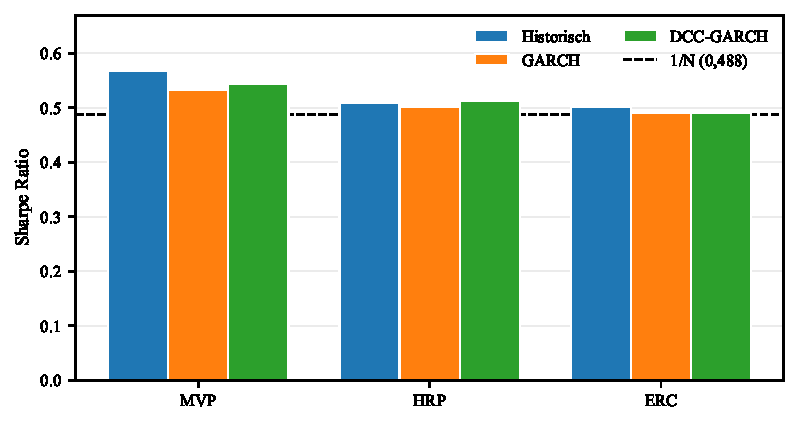
\includegraphics[width=0.88\textwidth]{Abbildungen/abb_sharpe_basis.pdf}
  \caption{Sharpe Ratio der Portfoliomodelle im Basisfall}
  \label{abb:sharpe_basis}
  \begin{minipage}{\linewidth}\vspace{0.4em}\centering\footnotesize
  TRBC, Training 1008 Handelstage, Prognosehorizont 1 Tag; die gestrichelte Linie markiert das 1/N-Portfolio.
  \end{minipage}
\end{figure}


Innerhalb der Portfoliomodelle kehrt sich die statistische Rangfolge im Basisfall weitgehend um, da bei MVP und ERC die historische Matrix vorne liegt und allein beim HRP der DCC-Schätzer marginal besser abschneidet.
Der GARCH-Schätzer bleibt dabei in allen drei Modellen hinter der historischen Matrix zurück.
Bei HRP und ERC senken die dynamischen Schätzer jedoch die realisierte Volatilität spürbar, während der DCC-Schätzer beim MVP auf einem ähnlichen Niveau wie der historische Schätzer liegt, wobei dieser Vorteil in der Sharpe Ratio durch die Einbindung der Rendite jeweils verschwindet.
Genau diese Größe schlagen \textcite{engle2006} für das Minimum-Varianz-Portfolio als ökonomisches Auswahlkriterium vor, da dessen realisierte Volatilität unmittelbar von der Kovarianzmatrix abhängt und nicht von den Renditen überlagert wird.
Diese Idee kann auch auf HRP und ERC übertragen werden, da deren Gewichte ebenfalls allein aus der Kovarianzmatrix stammen.

Gleichzeitig fällt der mittlere Turnover des MVP mit der DCC- wie auch mit der GARCH-Kovarianz rund 32-mal so hoch aus wie mit der historischen, wodurch beide dynamischen Schätzer bei einer realen Umsetzung nochmals schlechter abschneiden würden.
Grund für den hohen Turnover ist, dass die beiden dynamischen Modelle deutlich schneller auf Änderungen in der Volatilität reagieren, wodurch auch die Gewichtsverteilung der Portfolios angepasst wird, während die träge Stichprobenkovarianz die Gewichte nahezu unverändert lässt.
Bei HRP und ERC fällt der Anstieg mit dem Faktor 5 bis 8 erheblich geringer aus, was auf die robustere Konstruktion der beiden Modelle zurückzuführen ist.

Wie unterschiedlich die Verfahren das Kapital verteilen, zeigt die durchschnittliche Zahl der Sektoren mit einem Gewicht von mehr als 1\,\% in \hyperref[tab:oekonomie_basis]{Tabelle~\ref*{tab:oekonomie_basis}}. Das MVP konzentriert sich im Mittel auf nur vier bis fünf der rund 18 investierbaren Sektoren, während HRP und ERC nahezu alle Sektoren nennenswert gewichten. Diese deutlich breitere Streuung trägt letztlich zur höheren Robustheit von HRP und ERC bei.

Statistisch abgesichert sind die Unterschiede in der Sharpe Ratio allerdings nicht, da \hyperref[tab:jobson_korkie]{Tabelle~\ref*{tab:jobson_korkie}} für keinen der relevanten Vergleiche einen auch nur annähernd signifikanten $p$-Wert ausweist.
Dies gilt sowohl zwischen den Kovarianzschätzern als auch gegenüber dem 1/N-Portfolio.

% automatisch erzeugt von paper/tabellen.py -- nicht von Hand editieren
\begin{table}[htbp]
  \centering
  \footnotesize
  \begin{tabular}{lrrr@{}l}
    \toprule
    Vergleich & $\Delta$ Sharpe & $z$-Statistik & \multicolumn{2}{c}{$p$-Wert} \\
    \midrule
    MVP Historical vs.\ MVP GARCH & 0,0352 & 0,55 & 0,584 &  \\
    MVP Historical vs.\ MVP DCC & 0,0243 & 0,37 & 0,709 &  \\
    MVP GARCH vs.\ MVP DCC & -0,0109 & -0,78 & 0,435 &  \\
    HRP Historical vs.\ HRP GARCH & 0,0063 & 0,30 & 0,764 &  \\
    HRP Historical vs.\ HRP DCC & -0,0041 & -0,18 & 0,859 &  \\
    HRP GARCH vs.\ HRP DCC & -0,0104 & -1,23 & 0,220 &  \\
    ERC Historical vs.\ ERC GARCH & 0,0105 & 0,95 & 0,342 &  \\
    ERC Historical vs.\ ERC DCC & 0,0111 & 0,98 & 0,329 &  \\
    ERC GARCH vs.\ ERC DCC & 0,0006 & 0,27 & 0,784 &  \\
    MVP Historical vs.\ Naive & 0,0797 & 0,69 & 0,487 &  \\
    HRP Historical vs.\ Naive & 0,0210 & 0,66 & 0,509 &  \\
    ERC Historical vs.\ Naive & 0,0132 & 0,85 & 0,395 &  \\
    \bottomrule
  \end{tabular}
  \caption{Tests auf Unterschiede der Sharpe Ratios (Basisfall)}
  \label{tab:jobson_korkie}
  \begin{minipage}{\linewidth}\vspace{0.4em}\centering\footnotesize
  Auf Überschussrenditen über die Fed Funds Rate; $^{***}$, $^{**}$, $^{*}$ = 1-, 5-, 10-\%-Niveau.
  \end{minipage}
\end{table}


Die Auswirkungen proportionaler Transaktionskosten sind in \hyperref[tab:transaktionskosten]{Tabelle~\ref*{tab:transaktionskosten}} im \hyperref[sec:anhang_kosten]{Anhang~\ref*{sec:anhang_kosten}} dargestellt.
Bereits bei 5~Basispunkten auf das umgeschlagene Volumen fällt die Sharpe Ratio des MVP mit DCC-Kovarianz von 0,543 auf 0,310 und liegt damit deutlich unter dem naiven Portfolio mit 0,484, während die historische Variante mit 0,560 nahezu unverändert bleibt.
Bei 20~Basispunkten werden beide dynamischen MVP-Varianten negativ.

\hyperref[tab:bilanz]{Tabelle~\ref*{tab:bilanz}} fasst die Ergebnisse über alle 40~Kombinationen aus Trainingsfenster und Prognosehorizont zusammen, wobei je Portfoliomodell angegeben wird, wie oft das 1/N-Portfolio geschlagen wird und wie oft die dynamischen Schätzer die historische Matrix übertreffen.
Bewertungsmaßstab ist dabei die Sharpe Ratio, wobei der Befund je nach Portfoliomodell unterschiedlich ausfällt.
Zur ersten Forschungsfrage zeigt sich, dass HRP und ERC mit historischer Kovarianz das 1/N-Portfolio in rund 90 Prozent der Konstellationen schlagen, das MVP dagegen nur in einem Fünftel der Fälle.
Ausschlaggebend ist die bereits angelegte Anfälligkeit des MVP, dass Schätzfehler im Optimierungsprozess verstärkt werden, wodurch konzentrierte Portfolios entstehen.
Die im Basisfall beste Sharpe Ratio des MVP ist insofern nicht repräsentativ.

Zur zweiten Forschungsfrage zeigt sich ein klares Muster entlang der Portfoliomodelle, da die dynamischen Schätzer die historische Matrix beim MVP in mehr als der Hälfte der Läufe schlagen, beim HRP nur vereinzelt und beim ERC in keinem einzigen.
Ökonomisch ist das gut erklärbar, weil das MVP als einziges Verfahren die Kovarianzmatrix vollständig einschließlich ihrer Inversen ausnutzt, während HRP lediglich die Clusterordnung und die Varianzen der Teilcluster verwendet und ERC die Risikobeiträge ausbalanciert.
Eine bessere Kovarianzprognose zahlt sich folglich dort aus, wo sie am intensivsten genutzt wird, und bleibt folgenlos, wo das Verfahren die Matrix nur grob verwendet.
Somit steht das ökonomische Ergebnis im Gegensatz zum statistischen Befund.

% automatisch erzeugt von paper/tabellen.py -- nicht von Hand editieren
\begin{table}[htbp]
  \centering
  \footnotesize
  \begin{tabular}{llrrrr}
    \toprule
    Modell & Kovarianz & vs.\ 1/N & \multicolumn{3}{c}{vs.\ historische Matrix} \\
    \cmidrule(lr){4-6}
     & & Sharpe & Sharpe & QLIKE & MSE \\
    \midrule
    MVP & Historisch & 20/40 & -- & -- & -- \\
    MVP & GARCH & 19/40 & 22/40 & 36/40 & 40/40 \\
    MVP & DCC-GARCH & 20/40 & 25/40 & 37/40 & 40/40 \\
    \midrule
    HRP & Historisch & 40/40 & -- & -- & -- \\
    HRP & GARCH & 32/40 & 3/40 & 36/40 & 40/40 \\
    HRP & DCC-GARCH & 31/40 & 3/40 & 37/40 & 40/40 \\
    \midrule
    ERC & Historisch & 40/40 & -- & -- & -- \\
    ERC & GARCH & 31/40 & 0/40 & 36/40 & 40/40 \\
    ERC & DCC-GARCH & 32/40 & 0/40 & 37/40 & 40/40 \\
    \bottomrule
  \end{tabular}
  \caption{Ergebnisse über alle empirischen Läufe}
  \label{tab:bilanz}
  \begin{minipage}{\linewidth}\vspace{0.4em}\centering\footnotesize
  Alle 40 Kombinationen aus Trainingsfenster und Prognosehorizont, bewertet ab 01.01.2010.
  \end{minipage}
\end{table}


Auch über die Trainingsfenster hinweg bleibt dieses Muster erhalten (\hyperref[abb:sharpe_train]{siehe Abb.~\ref*{abb:sharpe_train}}).
Beim MVP liegt DCC in allen zehn Fenstern über der historischen Matrix, bei HRP in einem und bei ERC in keinem.
Der GARCH-Schätzer folgt diesem Muster bei HRP und ERC, erreicht beim MVP mit sechs von zehn Fenstern aber einen deutlich schwächeren Vorsprung als DCC.
Dass DCC hier beim MVP vorne liegt, während im Basisfall die historische Matrix führt, ist kein Widerspruch, sondern ein Zeitraumeffekt, da diese Vergleiche auf dem gemeinsamen Zeitraum ab 2010 beruhen und das MVP mit dynamischer Kovarianz gerade in der Phase 2010--2019 vorne liegt (\hyperref[sec:anhang_strukturbruch]{siehe Anhang~\ref*{sec:anhang_strukturbruch}}).
Die absoluten Unterschiede fallen dabei klein aus, weshalb angesichts der insignifikanten Tests auf Sharpe-Differenzen keine belastbare Rangfolge abgeleitet werden sollte.

%% automatisch erzeugt von paper/tabellen.py -- nicht von Hand editieren
\begin{table}[htbp]
  \centering
  \footnotesize
  \begin{tabular}{rrrrrrrrrrr}
    \toprule
    Training & \multicolumn{3}{c}{MVP} & \multicolumn{3}{c}{HRP} & \multicolumn{3}{c}{ERC} & 1/N \\
    \cmidrule(lr){2-4}\cmidrule(lr){5-7}\cmidrule(lr){8-10}
     & Hist. & GARCH & DCC & Hist. & GARCH & DCC & Hist. & GARCH & DCC & \\
    \midrule
    252 & 0,628 & 0,612 & 0,625 & 0,695 & 0,677 & 0,665 & 0,685 & 0,676 & 0,674 & 0,676 \\
    504 & 0,605 & 0,735 & 0,741 & 0,696 & 0,700 & 0,690 & 0,688 & 0,682 & 0,681 & 0,685 \\
    756 & 0,633 & 0,668 & 0,672 & 0,695 & 0,683 & 0,685 & 0,689 & 0,678 & 0,678 & 0,676 \\
    1008 & 0,714 & 0,706 & 0,728 & 0,684 & 0,686 & 0,706 & 0,692 & 0,680 & 0,682 & 0,677 \\
    1260 & 0,721 & 0,699 & 0,729 & 0,686 & 0,669 & 0,672 & 0,675 & 0,663 & 0,665 & 0,656 \\
    1512 & 0,681 & 0,669 & 0,696 & 0,685 & 0,667 & 0,669 & 0,675 & 0,663 & 0,665 & 0,660 \\
    1764 & 0,642 & 0,670 & 0,686 & 0,656 & 0,641 & 0,649 & 0,642 & 0,634 & 0,636 & 0,621 \\
    2016 & 0,631 & 0,652 & 0,655 & 0,657 & 0,649 & 0,647 & 0,650 & 0,644 & 0,645 & 0,628 \\
    2268 & 0,657 & 0,689 & 0,683 & 0,671 & 0,653 & 0,656 & 0,661 & 0,654 & 0,655 & 0,635 \\
    2520 & 0,627 & 0,690 & 0,689 & 0,679 & 0,663 & 0,660 & 0,669 & 0,661 & 0,662 & 0,647 \\
    \bottomrule
  \end{tabular}
  \caption{Sharpe Ratios über die Trainingsfenster (TRBC, $h=1$)}
  \label{tab:sharpe_train}
  \begin{minipage}{\linewidth}\vspace{0.4em}\centering\footnotesize
  Annualisierte Sharpe Ratio ($r_f=0$), bewertet ab 01.01.2010.
  \end{minipage}
\end{table}


% automatisch erzeugt von paper/abbildungen.py -- nicht von Hand editieren
\begin{figure}[htbp]
  \centering
  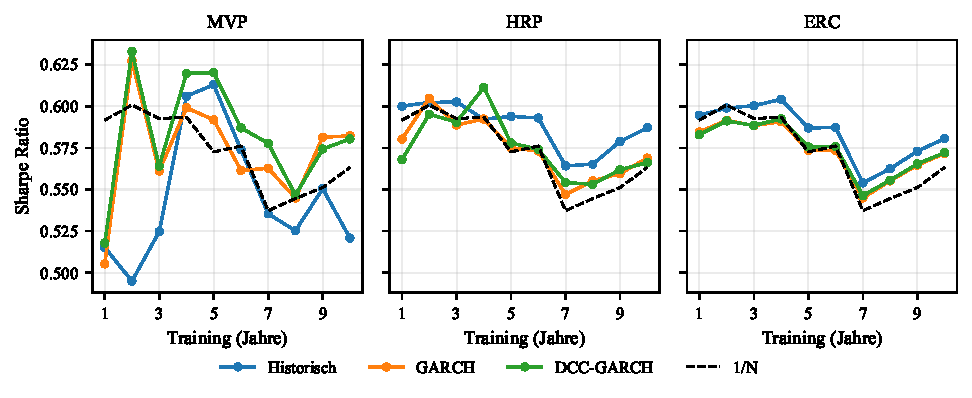
\includegraphics[width=\textwidth]{Abbildungen/abb_sharpe_train.pdf}
  \caption{Sharpe Ratio über die Trainingsfenster}
  \label{abb:sharpe_train}
  \begin{minipage}{\linewidth}\vspace{0.4em}\centering\footnotesize
  TRBC, Prognosehorizont 1 Tag, Bewertung ab 01.01.2010 für alle Fenster.
  \end{minipage}
\end{figure}


Deutlicher ist der Befund über den Prognosehorizont in \hyperref[tab:sharpe_horizont]{Tabelle~\ref*{tab:sharpe_horizont}}.
Der tägliche Basisfall dient dabei vor allem dazu, den Effekt der Kovarianzdynamik ohne die Nebenwirkungen seltenerer Rebalancierung zu isolieren, jedoch werden in der Realität auch längere Rebalancierungszyklen relevant.
Wird seltener rebalanciert, bleibt die Sharpe Ratio der historischen Matrix beim MVP praktisch konstant, während sie für DCC und ebenso für GARCH bei den beiden längeren Horizonten deutlich fällt und der Turnover je Rebalancierung gleichzeitig auf mehr als das Doppelte steigt.
Der Verlauf ist dabei nicht monoton, da beide dynamischen Schätzer bei einem Horizont von fünf Tagen zunächst ihren höchsten Wert im gesamten Feld erreichen und erst danach zurückfallen.
Eine Erklärung hierfür ist, dass sich die historisch geschätzte Kovarianzmatrix nur langsam mit der Zeit verändert, weshalb ihre Prognose schon bei kurzen Vorhersagezeiträumen keine aktuelle Dynamik abbildet und über eine längere Halteperiode entsprechend wenig veraltet.
Die GARCH-Modelle hingegen reflektieren Abweichungen nahezu sofort, weshalb ihre Prognose zwar den Formationszeitpunkt genau trifft, über die Halteperiode hinweg aber schnell veraltet.
Das Maximum bei fünf Tagen deutet darauf hin, dass ein Teil der täglichen Umschichtungen auf Schätzrauschen und nicht auf verwertbare Dynamik reagiert, sodass dessen Wegfall die Performance zunächst verbessert, bevor das Veralten der Prognose überwiegt.
Erkennbar ist das auch am Turnover, da dessen hohes Niveau anzeigt, wie stark sich die Kovarianzmatrix der dynamischen Modelle über eine längere Halteperiode verändert.
Aufgrund der selteneren Rebalancierung fällt der über die gesamte Historie kumulierte Turnover trotz des höheren Werts je Rebalancierung jedoch geringer aus, womit auch die Kostenbelastung einer realen Umsetzung sinken würde.
Bei HRP und ERC bleiben die Sharpe Ratios hingegen weitestgehend stabil, was wiederum auf die Robustheit dieser Verfahren hindeutet.

% automatisch erzeugt von paper/tabellen.py -- nicht von Hand editieren
\begin{table}[htbp]
  \centering
  \footnotesize
  \begin{tabular}{rrrrrrrrrr}
    \toprule
    $h$ (Tage) & \multicolumn{2}{c}{MVP} & \multicolumn{2}{c}{HRP} & \multicolumn{2}{c}{ERC} & 1/N & \multicolumn{2}{c}{Turnover MVP} \\
    \cmidrule(lr){2-3}\cmidrule(lr){4-5}\cmidrule(lr){6-7}\cmidrule(lr){9-10}
     & Hist. & DCC & Hist. & DCC & Hist. & DCC & & Hist. & DCC \\
    \midrule
    1 & 0,714 & 0,728 & 0,684 & 0,706 & 0,692 & 0,682 & 0,677 & 0,008 & 0,255 \\
    5 & 0,705 & 0,762 & 0,681 & 0,690 & 0,694 & 0,684 & 0,680 & 0,021 & 0,522 \\
    10 & 0,717 & 0,654 & 0,692 & 0,670 & 0,698 & 0,680 & 0,684 & 0,033 & 0,598 \\
    21 & 0,721 & 0,640 & 0,697 & 0,689 & 0,700 & 0,689 & 0,685 & 0,058 & 0,587 \\
    \bottomrule
  \end{tabular}
  \caption{Sharpe Ratios und Turnover über die Prognosehorizonte (TRBC, Training 1008 Tage)}
  \label{tab:sharpe_horizont}
  \begin{minipage}{\linewidth}\vspace{0.4em}\centering\footnotesize
  Annualisierte Sharpe Ratio ($r_f=0$), bewertet ab 01.01.2010; Turnover je Rebalancierung, also nicht auf gleiche Frequenz normiert.
  \end{minipage}
\end{table}


% =============================================================================
\section{Einordnung in die Literatur}\label{sec:literatur}
\iffalse
% [Vorschlag 1.2/5.2] TODO abgearbeitet: Raffinot (2018a/b) und López de Prado
% (2019) zu HERC/NCO sowie Jain und Jain (2019) zu DCC in risikobasierten
% Portfolios sind unten im Text ergänzt.
% ursprüngliches TODO (zur Referenz):
% TODO: Zu ergaenzen sind aktuelle Arbeiten zu HRP-Varianten (HERC, NCO) sowie
% zur Kombination von DCC-Modellen mit Risk-Parity-Ansaetzen.

In diesem Abschnitt werden die Befunde in die eingangs skizzierte Literatur eingeordnet.

Der Befund, dass alle drei risikobasierten Verfahren das naive Portfolio im Basisfall übertreffen, steht in Spannung zu \textcite{demiguel2009}, die 1/N gegenüber optimierten Strategien als schwer zu schlagen ausweisen.
Die Ursache dürfte weniger in den Verfahren als im Untersuchungsobjekt liegen, da hier über breit diversifizierte Sektorindizes statt über Einzeltitel optimiert wird und die Kovarianzmatrix dadurch stabiler zu schätzen ist.
Innerhalb der risikobasierten Verfahren fügen sich die Ergebnisse dagegen gut in die vorliegende Evidenz ein.
Die hohe Robustheit von HRP mit 35 von 40 Läufen über 1/N entspricht den Aussagen von \textcite{deprado2016} und \textcite{sen2022}.
\neu{Nachfolgende Arbeiten wie \textcite{raffinot2018hcaa} und \textcite{raffinot2018herc} verfeinern den hierarchischen Ansatz um alternative Clusterverfahren und eine risikoparitätische statt rein varianzbasierte Aufteilung innerhalb der Cluster, und \textcite{deprado2019nco} löst mit der Nested-Clustered-Optimization das der HRP zugrunde liegende Instabilitätsproblem auf andere Weise. Die vorliegende Arbeit beschränkt sich auf die ursprüngliche HRP-Variante von \textcite{deprado2016} und öffnet diese Erweiterungen als Ansatzpunkt für weitere Untersuchungen.}
Mit \textcite{chaves2011} deckt sich zudem die Beobachtung, dass ERC zwar besser diversifiziert, das naive Portfolio aber nicht durchgängig schlägt.
Dass das MVP im Basisfall dennoch die höchste Sharpe Ratio erzielt, über alle Läufe hinweg aber nur in einem Fünftel der Fälle über 1/N liegt, illustriert genau die Instabilität, die \textcite{lee2011} und \textcite{behr2008} beschreiben.

Das zentrale Ergebnis dieser Arbeit ist ein nahezu vollständiger statistischer, aber nur beim MVP nennenswerter ökonomischer Vorsprung der GARCH-Modelle.
Die durchweg insignifikanten Tests in \hyperref[tab:jobson_korkie]{Tabelle~\ref*{tab:jobson_korkie}} bestätigen den Einwand von \textcite{engle2006} für den vorliegenden Datensatz unmittelbar, während die von \textcite{patton2011} und \textcite{laurent2013} vorgeschlagenen robusten Verluste im selben Datensatz sehr wohl trennscharf sind.
Nur scheinbar im Widerspruch dazu stehen \textcite{ardia2017}, die eine Fehlspezifikation der Kovarianzmatrix als spürbare Verzerrung der Portfoliogewichte ausweisen.
Verzerrte Gewichte schlagen sich hier nur dort in der Performance nieder, wo ein Verfahren die Matrix intensiv nutzt, sodass sich beide Befunde nicht ausschließen, sondern die Verzerrung je nach Allokationsverfahren unterschiedlich teuer ist.
Am nächsten liegt jedoch \textcite{moura2020}, da die Autoren für hochdimensionale bedingte Kovarianzmatrizen ebenfalls finden, dass die statistisch beste Spezifikation nicht die ökonomisch beste sein muss und Transaktionskosten den Ausschlag geben.
Der um ein Vielfaches erhöhte Turnover der dynamischen Schätzer zeigt denselben Mechanismus in einem Sektoruniversum.
\neu{Für risikobasierte Portfolios speziell mit DCC-GARCH-Kovarianz finden \textcite{jain2019}, dass multivariate GARCH-Schätzer robuster gegenüber Kovarianzfehlspezifikation sind als der Stichprobenschätzer und sich der DCC-Schätzer gerade in kleinen Anlageuniversen auszeichnet. Das deckt sich mit dem hier für HRP und ERC beobachteten, wenn auch ökonomisch folgenlosen statistischen Vorsprung der dynamischen Schätzer.}

% =============================================================================
\fi
\section{Limitationen}\label{sec:limitationen}
\iffalse
Die Aussagekraft der Ergebnisse ist in mehrfacher Hinsicht begrenzt, wobei die Einschränkungen im Folgenden nach ihrem Gewicht für die Interpretation geordnet werden.

Eine zentrale Limitation ist dabei, dass der Backtest ohne Handelskosten rechnet und Kosten nur nachträglich als proportionaler Abschlag berücksichtigt werden, obwohl sich die Verfahren im Turnover um den Faktor~32 unterscheiden.
Die berichteten Kennzahlen begünstigen damit die dynamischen Schätzer, deren Nachteil unter realen Kosten größer ausfiele als ausgewiesen.
Umgekehrt wird die Aussage des \hyperref[sec:oekonomisch]{Abschnitts zur ökonomischen Performance} dadurch nicht geschwächt, sondern verschärft, da dieser Nachteil bereits ohne Kosten vorhanden ist.

Auf der Messseite ist der realisierte Proxy die wesentliche Einschränkung, da er für $h = 1$ aus einem einzigen äußeren Produkt besteht und damit den Rang eins hat.
Beide Verlustfunktionen bleiben nach \textcite{patton2011} und \textcite{laurent2013} unabhängig von der Genauigkeit des Proxys rangerhaltend, jedoch begrenzt das geringe Signal-Rausch-Verhältnis die Teststärke des DM-Tests, wobei der MSE stärker betroffen ist als der QLIKE-Verlust.
Intraday-Daten würden einen erheblich präziseren Proxy liefern, standen für diese Arbeit aber nicht zur Verfügung.
Hinzu kommt, dass ausschließlich die relative Prognosegüte bewertet wurde und nicht die absolute Kalibrierung der prognostizierten Volatilität.
Ob die Modelle das Risikoniveau im Mittel treffen, bleibt damit offen.

Des Weiteren beruht die gesamte Auswertung auf einem einzigen Universum, dessen Sektorindizes rechnerische Größen sind und sich nicht unmittelbar handeln lassen, weshalb eine direkte Replikation der optimierten Portfolios nicht möglich ist.
Gezeigt ist damit, dass die Befunde für diese Datengrundlage gelten, nicht aber, ob sie sich auf andere Märkte übertragen lassen.

% [Vorschlag 2.1] Limitation zu 260 vs. 252 Handelstagen/Jahr auf Wunsch
% wieder entfernt, siehe Kommentar in Abschnitt 2.1.
%\neu{Auf der Datenseite enthalten die Sektorreihen Feiertage als Handelstage mit Nullrendite, da Datastream sie mit dem Kurs des Vortages auffüllt (\hyperref[sec:daten]{Abschnitt~\ref*{sec:daten}}).
%Das drückt die geschätzten Varianzen und Korrelationen geringfügig und lässt die 252er-Annualisierung nicht exakt auf die tatsächlichen rund 260 Handelstage pro Jahr passen; da beides alle Kovarianzschätzer und Portfoliomodelle gleichermaßen betrifft, verschiebt es aber keine der berichteten Rangfolgen.}

% Das eher Erweiterung
%Auf der Modellseite wird ausschließlich GARCH(1,1) unter Normalverteilungsannahme geschätzt, obwohl diese Annahme in der Realität nicht standhält.
%Zudem zeigt sich in empirischen Untersuchungen, dass negative Shocks in der Regel einen stärkeren Einfluss auf die nachfolgende Volatilität haben als positive Shocks.
%Anderes als das einfache GARCH-Model, binden Modelle wie GJR-GARCH und EGARCH diese Asymmetrie mit ein und sind somit realitätsnäher.
% -> jetzt ausformuliert unten in 6.1 Ausblick, inkl. Bollerslev/Wooldridge (1992)
\fi

\subsection{Ausblick}\label{sec:forschung}
Aus den Ergebnissen und den genannten Einschränkungen ergeben sich vier Ansatzpunkte für weitere Untersuchungen.

Auf der Modellseite wird ausschließlich ein GARCH(1,1) geschätzt, obwohl dieses Modell im Vergleich zur Realität vereinfachte Annahmen trifft.
Beispielsweise zeigt sich in empirischen Untersuchungen, dass negative Schocks in der Regel einen stärkeren Einfluss auf die nachfolgende Volatilität haben als positive.
Anders als das einfache GARCH-Modell binden Modelle wie GJR-GARCH und EGARCH diese Asymmetrie ein und sind somit realitätsnäher, während sich über höhere Ordnungen oder ein GARCH-MIDAS zusätzlich längerfristige Komponenten der Volatilität erfassen lassen.
Da der ökonomische Nachteil der dynamischen Schätzer hier hauptsächlich aus dem Turnover und nicht aus der Prognosegüte stammt, wäre allerdings zu prüfen, ob eine realitätsnähere Varianzdynamik daran überhaupt etwas ändert.

Auf der Allokationsseite ließe sich das Feld um modernere Verfahren wie Hierarchical Equal Risk Contribution \parencite{raffinot2018herc} oder Nested Clustered Optimization \parencite{deprado2019nco} erweitern, die die hierarchische Struktur von HRP anders auswerten.
Beide nutzen die Kovarianzmatrix intensiver als HRP, ohne sie wie das MVP vollständig zu invertieren.
Da sich der Mehrwert einer besseren Prognose in dieser Arbeit genau danach richtet, wie intensiv ein Verfahren die Matrix nutzt, ließe sich an ihnen prüfen, ob der Zusammenhang auch auf den Stufen dazwischen gilt.
Offen bleibt zudem, ob eine bessere Kovarianzmatrix in Verfahren, die zusätzlich eine Renditeprognose verwenden, einen größeren Vorteil liefert, da die Matrix dort nicht nur das Risiko begrenzt, sondern auch die Gewichtung der erwarteten Renditen bestimmt.

Der dritte Ansatzpunkt betrifft die Transaktionskosten, die hier weder im Backtest noch in der Optimierung berücksichtigt werden.
Ein kostenbewusster Optimierer würde den Turnover in die Zielfunktion aufnehmen und dadurch einen Teil der Belastung vermeiden, statt sie nur zu erleiden.
Ob die dynamischen Schätzer unter einer solchen Nebenbedingung weiterhin zurückfallen, ist offen und wäre für die praktische Bewertung der entscheidende Test.

Schließlich sollten die Befunde an weiteren Datensätzen überprüft werden, etwa an Einzeltiteln, anderen Regionen oder Anlageklassen mit geringerer durchschnittlicher Korrelation.
Gerade die hohe paarweise Korrelation des hier verwendeten Universums begrenzt die Diversifikationsmöglichkeiten von vornherein und könnte den Spielraum für eine bessere Kovarianzprognose systematisch verengen.

% =============================================================================
\section{Fazit}\label{sec:fazit}
Die Arbeit hat zwei Fragen getrennt untersucht, nämlich ob risikobasierte Portfoliomodelle das naive 1/N-Portfolio schlagen und ob GARCH-basierte Kovarianzprognosen gegenüber der historischen Schätzung einen Mehrwert stiften.

Zur ersten Frage hängt die Antwort stark vom gewählten Verfahren ab.
HRP und ERC mit historischer Kovarianz übertreffen das 1/N-Portfolio in rund neun von zehn untersuchten Konstellationen und erweisen sich als robust gegenüber Variationen von Trainings- und Prognosefenster.
Das Minimum-Varianz-Portfolio erzielt im Basisfall zwar die höchste Sharpe Ratio, schlägt 1/N über alle Läufe hinweg aber nur in einem Fünftel der Fälle und reagiert am empfindlichsten auf Schätzfehler.
Für die Praxis sprechen diese Ergebnisse damit eher für die robusteren Verfahren als für die Varianzminimierung, wobei einschränkend gilt, dass keiner der Vorsprünge gegenüber 1/N statistisch signifikant ist.

Zur zweiten Frage entscheidet das angelegte Kriterium über die Antwort, worin zugleich der Hauptbefund liegt.
Statistisch ist das Ergebnis eindeutig, da DCC-GARCH die Kovarianzmatrix in allen 40~Läufen unter dem MSE und in nahezu allen unter dem QLIKE-Verlust besser prognostiziert als die historische Schätzung und die Abstände zur historischen Matrix im DM-Test signifikant sind.
Ökonomisch schlägt sich dieser Vorsprung jedoch nur dort nieder, wo die Kovarianzmatrix tatsächlich intensiv genutzt wird, also beim MVP und nicht bei HRP oder ERC.
Das ist konsistent mit der Konstruktion der Verfahren, da beide die Matrix nur grob nutzen und gerade deshalb robust, zugleich aber auch unempfindlich gegenüber ihrer Verbesserung sind.
Der Preis der Dynamik ist der Turnover, der beim MVP um den Faktor~32 höher liegt und den ohnehin geringen Vorsprung unter realen Handelskosten aufzehren würde.

Der übergreifende Schluss lautet damit, dass eine bessere Risikoprognose nicht automatisch eine bessere Anlageentscheidung ist.
Die GARCH-Modelle leisten das, wofür sie konstruiert sind, und die synthetische Validierung zeigt, dass sie genau dann einen Mehrwert liefern, wenn der datengenerierende Prozess ihre Annahmen erfüllt.
Selbst dann ist dieser Mehrwert jedoch nicht garantiert.
Im DCC-Datensatz aus \hyperref[sec:anhang_synth]{Anhang~\ref*{sec:anhang_synth}} liefert das korrekt spezifizierte DCC-Modell zwar in allen zehn Trainingsfenstern den besseren QLIKE-Verlust und die niedrigere realisierte Volatilität, unterliegt beim MVP-Sharpe aber in drei von zehn Fenstern dem falsch spezifizierten GARCH-Modell.
Prognosegüte und Anlageerfolg fallen somit bereits bei bekanntem datengenerierendem Prozess auseinander.
Auf realen Sektordaten ist die verwertbare Struktur jedoch zu schwach, um die Kosten der laufenden Umschichtung zu rechtfertigen.
Nicht die Prognosegüte ist folglich die bindende Restriktion, sondern der Handel, den ihre Nutzung auslöst.

\newpage
% =============================================================================
\appendix
\section{Voller und gemeinsamer Bewertungszeitraum}\label{sec:anhang_strukturbruch}
Sämtliche im Ergebnisteil berichteten Vergleiche über Trainingsfenster hinweg wurden auf dem gemeinsamen Zeitraum ab 2010 gerechnet.
Dieser Anhang begründet, warum diese Einschränkung nötig ist, und zeigt, was ohne sie gemessen würde.

Ohne die Einschränkung bewertet jedes Trainingsfenster einen anderen Zeitraum, da der Out-of-Sample-Beginn von März~2000 beim kürzesten auf November~2008 beim längsten Fenster wandert.
Der Lauf mit einem Jahr Training enthält damit das Platzen der Dotcom-Blase, während der Lauf mit zehn Jahren Training erst nach der Finanzkrise beginnt und nur die Erholung abdeckt, wodurch dessen Kennzahlen angehoben werden, ohne dass dies etwas über die Schätzqualität aussagt.
Wie stark der Effekt wiegt, zeigt \hyperref[abb:sharpe_zeitraum]{Abbildung~\ref*{abb:sharpe_zeitraum}}, in der die Sharpe Ratio über die Trainingsfenster einmal über die volle Historie und einmal über den gemeinsamen Zeitraum aufgetragen ist.
Der Sprung beim längsten Fenster tritt links auch beim 1/N-Portfolio auf, obwohl dieses überhaupt keine Schätzung vornimmt, und verschwindet rechts vollständig.
Es handelt sich somit um einen reinen Stichprobeneffekt.

% automatisch erzeugt von paper/abbildungen.py -- nicht von Hand editieren
\begin{figure}[htbp]
  \centering
  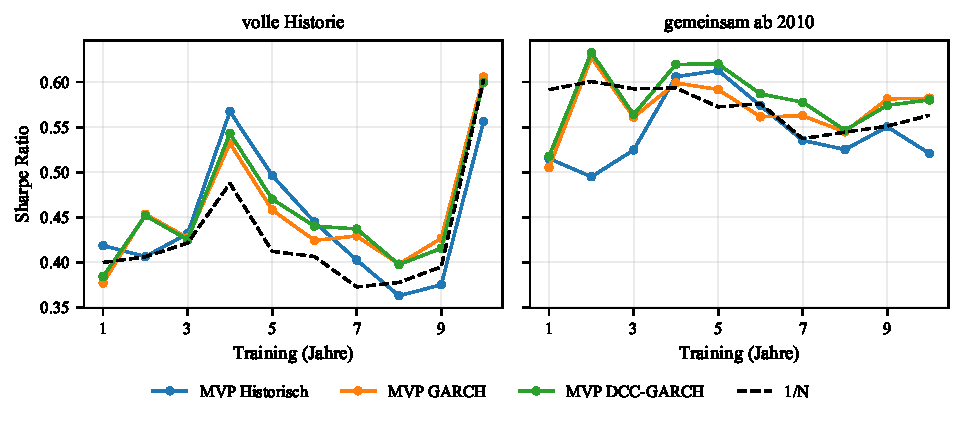
\includegraphics[width=\textwidth]{Abbildungen/abb_sharpe_zeitraum.pdf}
  \caption{Sharpe Ratio über die Trainingsfenster, voller und gemeinsamer Bewertungszeitraum}
  \label{abb:sharpe_zeitraum}
  \begin{minipage}{\linewidth}\vspace{0.4em}\centering\footnotesize
  TRBC, Prognosehorizont 1 Tag, links die volle Historie des jeweiligen Fensters, rechts der für alle Fenster identische Zeitraum ab 01.01.2010.
  \end{minipage}
\end{figure}


\hyperref[tab:strukturbruch_qlike]{Tabelle~\ref*{tab:strukturbruch_qlike}} und \hyperref[tab:strukturbruch_sharpe]{Tabelle~\ref*{tab:strukturbruch_sharpe}} stellen je Trainingsfenster die Kennzahlen über die volle Historie denen über den gemeinsamen Zeitraum ab 2010 gegenüber.
Die erste Tabelle weist neben der mittleren Größe des Anlageuniversums den QLIKE-Verlust der historischen Matrix und der beiden dynamischen Kovarianzschätzer aus, die zweite die Sharpe Ratio des MVP mit allen drei Kovarianzschätzern sowie die des 1/N-Portfolios.
Die 90-\%-Verfügbarkeitsregel lässt die zuletzt hinzugekommenen Sektoren in langen Fenstern erst spät oder gar nicht zu, weshalb die Fensterlänge über die Dimension der Kovarianzmatrix auch das QLIKE-Niveau mitbestimmt.

% automatisch erzeugt von paper/tabellen.py -- nicht von Hand editieren
\begin{table}[htbp]
  \centering
  \footnotesize
  \resizebox{\ifdim\width>\linewidth \linewidth\else \width\fi}{!}{%
  \begin{tabular}{rrrrrrrr}
    \toprule
    Training & $\varnothing\,N$ & \multicolumn{2}{c}{Historisch} & \multicolumn{2}{c}{GARCH} & \multicolumn{2}{c}{DCC-GARCH} \\
    \cmidrule(lr){3-4}\cmidrule(lr){5-6}\cmidrule(lr){7-8}
     & & voll & gem. & voll & gem. & voll & gem. \\
    \midrule
    252 & 20,3 & -161,5 & -176,1 & -161,8 & -175,9 & -162,0 & -176,1 \\
    504 & 19,7 & -159,2 & -171,0 & -160,4 & -171,4 & -160,8 & -171,8 \\
    756 & 19,1 & -156,0 & -165,2 & -157,9 & -166,1 & -158,4 & -166,8 \\
    1008 & 18,5 & -152,8 & -159,7 & -155,4 & -161,1 & -156,1 & -161,9 \\
    1260 & 17,9 & -149,1 & -154,3 & -152,2 & -156,1 & -153,1 & -157,1 \\
    1512 & 17,4 & -146,1 & -150,1 & -149,2 & -151,8 & -150,2 & -152,9 \\
    1764 & 16,9 & -143,0 & -146,0 & -145,9 & -147,7 & -147,0 & -148,8 \\
    2016 & 16,4 & -139,6 & -142,0 & -142,4 & -143,8 & -143,7 & -144,9 \\
    2268 & 16,2 & -138,3 & -140,6 & -141,0 & -142,5 & -142,3 & -143,7 \\
    2520 & 16,2 & -139,1 & -140,0 & -141,3 & -142,0 & -142,7 & -143,3 \\
    \bottomrule
  \end{tabular}
  }
  \caption{QLIKE über vollen und gemeinsamen Bewertungszeitraum (TRBC, $h=1$)}
  \label{tab:strukturbruch_qlike}
  \begin{minipage}{\linewidth}\vspace{0.4em}\centering\footnotesize
  \emph{voll} bezeichnet die volle Historie des jeweiligen Fensters, \emph{gem.} den gemeinsamen Zeitraum ab 01.01.2010. $\varnothing\,N$ ist die mittlere Zahl investierbarer Sektoren im gemeinsamen Zeitraum.
  \end{minipage}
\end{table}


% automatisch erzeugt von paper/tabellen.py -- nicht von Hand editieren
\begin{table}[htbp]
  \centering
  \footnotesize
  \resizebox{\ifdim\width>\linewidth \linewidth\else \width\fi}{!}{%
  \begin{tabular}{rrrrrrrrr}
    \toprule
    Training & \multicolumn{2}{c}{MVP Historisch} & \multicolumn{2}{c}{MVP GARCH} & \multicolumn{2}{c}{MVP DCC-GARCH} & \multicolumn{2}{c}{1/N} \\
    \cmidrule(lr){2-3}\cmidrule(lr){4-5}\cmidrule(lr){6-7}\cmidrule(lr){8-9}
     & voll & gem. & voll & gem. & voll & gem. & voll & gem. \\
    \midrule
    252 & 0,419 & 0,515 & 0,377 & 0,505 & 0,384 & 0,518 & 0,400 & 0,592 \\
    504 & 0,406 & 0,495 & 0,453 & 0,627 & 0,452 & 0,633 & 0,406 & 0,601 \\
    756 & 0,432 & 0,525 & 0,427 & 0,561 & 0,425 & 0,564 & 0,422 & 0,593 \\
    1008 & 0,567 & 0,606 & 0,532 & 0,599 & 0,543 & 0,620 & 0,488 & 0,594 \\
    1260 & 0,496 & 0,613 & 0,458 & 0,592 & 0,470 & 0,620 & 0,412 & 0,573 \\
    1512 & 0,445 & 0,574 & 0,424 & 0,562 & 0,440 & 0,587 & 0,407 & 0,576 \\
    1764 & 0,403 & 0,535 & 0,429 & 0,563 & 0,437 & 0,578 & 0,373 & 0,537 \\
    2016 & 0,363 & 0,525 & 0,398 & 0,545 & 0,398 & 0,547 & 0,378 & 0,545 \\
    2268 & 0,375 & 0,550 & 0,427 & 0,581 & 0,416 & 0,574 & 0,395 & 0,551 \\
    2520 & 0,556 & 0,521 & 0,606 & 0,582 & 0,600 & 0,580 & 0,603 & 0,563 \\
    \bottomrule
  \end{tabular}
  }
  \caption{Sharpe Ratio über vollen und gemeinsamen Bewertungszeitraum (TRBC, $h=1$)}
  \label{tab:strukturbruch_sharpe}
  \begin{minipage}{\linewidth}\vspace{0.4em}\centering\footnotesize
  \emph{voll} bezeichnet die volle Historie des jeweiligen Fensters, \emph{gem.} den gemeinsamen Zeitraum ab 01.01.2010. Ausgewiesen ist die annualisierte Sharpe Ratio.
  \end{minipage}
\end{table}


Wie oft welcher Schätzer über alle 40~Kombinationen vorne liegt, weist \hyperref[tab:bestzaehlung]{Tabelle~\ref*{tab:bestzaehlung}} aus, getrennt nach der Sharpe Ratio je Portfoliomodell und den beiden Verlustmaßen.
Dass die Rangfolge der Schätzer nicht am Basisfall hängt, zeigt sich dort deutlich, da unter beiden Verlustmaßen DCC-GARCH nahezu durchgängig vorne liegt, während ökonomisch bei HRP und ERC die historische Matrix dominiert.

% automatisch erzeugt von paper/tabellen.py -- nicht von Hand editieren
\begin{table}[htbp]
  \centering
  \footnotesize
  \begin{tabular}{lrrr}
    \toprule
    Kennzahl & Historisch & GARCH & DCC-GARCH \\
    \midrule
    Sharpe MVP & 14/40 & 6/40 & 20/40 \\
    Sharpe HRP & 36/40 & 1/40 & 3/40 \\
    Sharpe ERC & 40/40 & 0/40 & 0/40 \\
    \midrule
    QLIKE & 3/40 & 0/40 & 37/40 \\
    Kovarianz-MSE & 0/40 & 1/40 & 39/40 \\
    \bottomrule
  \end{tabular}
  \caption{Häufigkeit des besten Kovarianzschätzers je Kennzahl}
  \label{tab:bestzaehlung}
  \begin{minipage}{\linewidth}\vspace{0.4em}\centering\footnotesize
  Alle 40 Kombinationen aus Trainingsfenster und Prognosehorizont, bewertet ab 01.01.2010. Ausgewiesen ist, wie oft der jeweilige Schätzer die höchste Sharpe Ratio beziehungsweise den niedrigsten Verlust liefert.
  \end{minipage}
\end{table}


Zeitlich lokalisieren lässt sich der Bruch über die Teilperioden des Basisfalls in \hyperref[tab:strukturbruch_teilperioden]{Tabelle~\ref*{tab:strukturbruch_teilperioden}}.
Das QLIKE-Niveau springt ab 2022 deutlich nach unten, wobei dieser Sprung exakt mit der Erweiterung des Universums von 17 auf 25~Sektoren im September~2022 zusammenfällt.
Innerhalb der Periode 2022--2026 wächst das Universum anschließend nochmals von 25 auf 27~Sektoren, da zwei erst 2019 gestartete Reihen die 90-\%-Verfügbarkeitsregel im 1008-Tage-Fenster erst 2024 beziehungsweise Ende 2024 erfüllen.
Die Tabellenspanne 17--27 für diese Periode bildet somit beide Schritte ab.
Der MSE zeigt an dieser Stelle keinen vergleichbaren Bruch, folgt dafür aber dem Volatilitätsniveau der Periode und steigt in der Finanzkrise auf mehr als das Siebzigfache des Werts der ruhigen Phase 2003--2007.
Beide Kennzahlen sind über Perioden hinweg somit nur eingeschränkt vergleichbar, wenn auch aus unterschiedlichen Gründen.

% automatisch erzeugt von paper/tabellen.py -- nicht von Hand editieren
\begin{table}[htbp]
  \centering
  \footnotesize
  \begin{tabular}{llrrrrrrr}
    \toprule
    Periode & $N$ & \multicolumn{2}{c}{QLIKE} & \multicolumn{2}{c}{MSE ($\times 10^{-7}$)} & \multicolumn{3}{c}{Sharpe} \\
    \cmidrule(lr){3-4}\cmidrule(lr){5-6}\cmidrule(lr){7-9}
     & & Hist. & $\Delta$ DCC & Hist. & DCC & MVP Hist. & MVP DCC & 1/N \\
    \midrule
    2003--2007 & 16--16 & -143,5 & -3,79 & 0,28 & 0,23 & 1,490 & 1,485 & 1,087 \\
    2008--2009 & 16--16 & -119,7 & -11,50 & 21,03 & 16,72 & -0,200 & -0,294 & -0,092 \\
    2010--2019 & 16--17 & -146,1 & -1,75 & 0,79 & 0,60 & 0,940 & 1,036 & 0,760 \\
    2020--2021 & 17--17 & -133,1 & -7,15 & 20,18 & 15,88 & 0,446 & 0,427 & 0,836 \\
    2022--2026 & 17--27 & -205,1 & -0,69 & 1,79 & 1,70 & 0,578 & 0,462 & 0,461 \\
    \bottomrule
  \end{tabular}
  \caption{Teilperioden des Basisfalls: Universum, Prognosequalität und Performance}
  \label{tab:strukturbruch_teilperioden}
  \begin{minipage}{\linewidth}\vspace{0.4em}\centering\footnotesize
  $N$ ist die Spannweite der investierbaren Sektoren; QLIKE-Niveaus sind zwischen Perioden mit unterschiedlichem $N$ nicht vergleichbar.
  \end{minipage}
\end{table}


Aussagekräftig bleibt die Differenz zwischen den Schätzern innerhalb einer Periode, die erheblich variiert.
In der Finanzkrise 2008/09 und im COVID-Zeitraum fällt sie um ein Vielfaches größer aus als in den ruhigen Phasen.
Der Mehrwert der dynamischen Modellierung konzentriert sich damit auf Phasen mit ausgeprägten Volatilitätsschocks, in denen eine statische Matrix dem Risikoniveau am stärksten nachläuft.

Ökonomisch ist die Rangfolge ebenfalls periodenabhängig, da das MVP mit DCC-Kovarianz und ebenso mit GARCH-Kovarianz die historische Variante in der Phase 2010--2019 klar schlägt, in allen übrigen Teilperioden jedoch zurückliegt.
Der Basisfall umfasst die volle Historie ab 2003 und mittelt über gegenläufige Teilperioden, weshalb dort die historische Matrix vorne liegt, während die auf 2010 eingeschränkten Tabellen für das MVP zugunsten von DCC ausfallen.
Beide Rechnungen sind korrekt, messen aber Unterschiedliches, wobei die Unterschiede in beide Richtungen durchgängig insignifikant sind und daher keine starke Aussage zulassen.

\section{Transaktionskosten}\label{sec:anhang_kosten}
\hyperref[tab:transaktionskosten]{Tabelle~\ref*{tab:transaktionskosten} weist die Sharpe Ratios des Basisfalls nach Abzug proportionaler Transaktionskosten auf das je Rebalancierung umgeschlagene Volumen aus.}

% automatisch erzeugt von paper/tabellen.py -- nicht von Hand editieren
\begin{table}[htbp]
  \centering
  \footnotesize
  \begin{tabular}{llrrrrr}
    \toprule
    Modell & Kovarianz & Turnover & 0 Bp. & 5 Bp. & 10 Bp. & 20 Bp. \\
    \midrule
    MVP & Historisch & 0,008 & 0,695 & 0,688 & 0,680 & 0,666 \\
    MVP & GARCH & 0,258 & 0,658 & 0,425 & 0,192 & -0,274 \\
    MVP & DCC-GARCH & 0,255 & 0,671 & 0,438 & 0,205 & -0,261 \\
    \midrule
    HRP & Historisch & 0,012 & 0,614 & 0,605 & 0,595 & 0,577 \\
    HRP & GARCH & 0,072 & 0,611 & 0,555 & 0,499 & 0,388 \\
    HRP & DCC-GARCH & 0,094 & 0,622 & 0,548 & 0,474 & 0,327 \\
    \midrule
    ERC & Historisch & 0,006 & 0,601 & 0,596 & 0,592 & 0,584 \\
    ERC & GARCH & 0,034 & 0,592 & 0,568 & 0,543 & 0,494 \\
    ERC & DCC-GARCH & 0,034 & 0,591 & 0,567 & 0,542 & 0,492 \\
    \midrule
    1/N & -- & 0,006 & 0,581 & 0,577 & 0,573 & 0,565 \\
    \bottomrule
  \end{tabular}
  \caption{Sharpe Ratios nach proportionalen Transaktionskosten (Basisfall)}
  \label{tab:transaktionskosten}
  \begin{minipage}{\linewidth}\vspace{0.4em}\centering\footnotesize
  Sharpe Ratio ($r_f=0$) nach Abzug von $c$ Basispunkten auf das je Rebalancierung umgeschlagene Volumen.
  \end{minipage}
\end{table}


\section{Synthetische Validierung}\label{sec:anhang_synth}
Ob die Modelle korrekt implementiert sind, lässt sich an echten Daten nicht prüfen, da der wahre datengenerierende Prozess unbekannt ist.
Stattdessen werden drei simulierte Datensätze mit jeweils 20~Anlagen und 6.000~Handelstagen verwendet, die dieselbe unbedingte Risikostruktur besitzen (annualisierte Volatilitäten zwischen 15\,\% und 35\,\%, durchschnittliche Korrelation 0,35) und sich ausschließlich in der Dynamik der zweiten Momente unterscheiden.
Der Monte-Carlo-Datensatz enthält unabhängige Ziehungen mit konstanter Kovarianz, in denen die historische Matrix korrekt spezifiziert ist.
Beim GARCH-Datensatz kommt eine GARCH(1,1)-Dynamik je Anlage mit $\alpha = 0{,}08$ und $\beta = 0{,}90$ bei konstanter Korrelation hinzu, während der DCC-Datensatz zusätzlich eine DCC-Rekursion mit $a = 0{,}03$ und $b = 0{,}96$ enthält.
Obwohl die wahre bedingte Kovarianzmatrix hier bekannt wäre, wird die Prognosegüte auch in der Simulation gegen den realisierten Proxy aus \hyperref[eq:proxy]{Gleichung~\ref*{eq:proxy}} gemessen, damit die Ergebnisse mit denen auf den realen Daten vergleichbar sind.

Die Ergebnisse des Basisfalls zeigen \hyperref[tab:synth_basis]{Tabelle~\ref*{tab:synth_basis}} und die DM-Tests in \hyperref[tab:synth_dmw]{Tabelle~\ref*{tab:synth_dmw}}.
Im Monte-Carlo-Fall unterscheiden sich die drei Schätzer praktisch nicht, denn die Verlustdifferenz der dynamischen Schätzer gegenüber der historischen Matrix ist zwar signifikant, in der Höhe aber verschwindend gering.
Im GARCH-Fall schlagen beide dynamischen Schätzer die historische Matrix signifikant, auch in Sharpe Ratio und realisierter Volatilität, unterscheiden sich untereinander aber nicht, da die Korrelation dort konstant ist.
Erst im DCC-Fall ist DCC dem GARCH-Schätzer signifikant überlegen, sodass die Implementierung jeweils genau die Struktur erkennt, die tatsächlich vorhanden ist.

% automatisch erzeugt von paper/tabellen.py -- nicht von Hand editieren
\begin{table}[htbp]
  \centering
  \footnotesize
  \begin{tabular}{llrrrrr}
    \toprule
    Datensatz & Kovarianz & QLIKE & MSE ($\times 10^{-8}$) & Vola (\%) & Sharpe & Turnover \\
    \midrule
    Monte Carlo & Historisch & -154,50 & 7,04 & 11,92 & 1,011 & 0,011 \\
     & GARCH & -154,47 & 7,04 & 11,95 & 1,003 & 0,074 \\
     & DCC-GARCH & -154,47 & 7,04 & 11,95 & 1,002 & 0,075 \\
    \midrule
    GARCH-Sim. & Historisch & -154,23 & 7,84 & 11,37 & 0,869 & 0,010 \\
     & GARCH & -157,25 & 7,57 & 9,85 & 0,984 & 0,154 \\
     & DCC-GARCH & -157,25 & 7,57 & 9,85 & 0,984 & 0,154 \\
    \midrule
    DCC-Sim. & Historisch & -154,13 & 9,86 & 11,93 & 0,668 & 0,011 \\
     & GARCH & -157,02 & 9,19 & 9,62 & 0,907 & 0,160 \\
     & DCC-GARCH & -162,13 & 8,98 & 8,99 & 0,925 & 0,152 \\
    \bottomrule
  \end{tabular}
  \caption{Synthetische Validierung: Basisfall je Datengenerierungsprozess}
  \label{tab:synth_basis}
  \begin{minipage}{\linewidth}\vspace{0.4em}\centering\footnotesize
  20 simulierte Anlagen, Training 1008 Handelstage, Prognosehorizont 1 Tag; Performancekennzahlen für das MVP.
  \end{minipage}
\end{table}


% automatisch erzeugt von paper/tabellen.py -- nicht von Hand editieren
\begin{table}[htbp]
  \centering
  \footnotesize
  \begin{tabular}{lr@{}lrr@{}lrr@{}lr}
    \toprule
    Datensatz & \multicolumn{2}{c}{$\Delta$ G--H} & $t$ & \multicolumn{2}{c}{$\Delta$ D--H} & $t$ & \multicolumn{2}{c}{$\Delta$ D--G} & $t$ \\
    \midrule
    Monte Carlo & 0,029 & $^{***}$ & 6,07 & 0,029 & $^{***}$ & 6,12 & 0,000 &  & 0,32 \\
    GARCH-Sim. & -3,025 & $^{***}$ & -24,69 & -3,024 & $^{***}$ & -24,68 & 0,000 &  & 1,28 \\
    DCC-Sim. & -2,887 & $^{***}$ & -15,64 & -7,998 & $^{***}$ & -35,68 & -5,111 & $^{***}$ & -49,85 \\
    \bottomrule
  \end{tabular}
  \caption{Synthetische Validierung: DMW-Tests auf die QLIKE-Differenzen}
  \label{tab:synth_dmw}
  \begin{minipage}{\linewidth}\vspace{0.4em}\centering\footnotesize
  G = GARCH, D = DCC-GARCH, H = historisch; negative Differenzen bedeuten eine bessere Prognose. $^{***}$, $^{**}$, $^{*}$ = 1-, 5-, 10-\%-Niveau.
  \end{minipage}
\end{table}


Wie stabil dieses Bild über die Länge des Trainingsfensters ist, zeigt \hyperref[tab:synth_stabilitaet]{Tabelle~\ref*{tab:synth_stabilitaet}}.
Da das Universum konstant 20~Anlagen umfasst und die Parameter des Prozesses über die gesamte Stichprobe unverändert bleiben, verschiebt sich das Niveau der Prognosekennzahlen kaum, denn das QLIKE-Niveau der historischen Matrix schwankt über alle zehn Fenster um höchstens gut zwei Punkte und das MSE-Niveau bleibt praktisch konstant.
Auch die Rangfolge kehrt sich in keinem Fenster um, da DCC in allen 20~Läufen unter beiden Verlustmaßen besser prognostiziert als die historische Matrix.

Der Vorsprung der dynamischen Schätzer wächst dabei mit der Länge des Trainingsfensters und stabilisiert sich erst bei den längeren Fenstern.
Im DCC-Datensatz steigt der QLIKE-Abstand zwischen DCC und historischer Matrix von 4,1~Punkten bei einem Jahr Training auf 8,5~Punkte bei zehn Jahren, im GARCH-Datensatz von 2,1 auf 2,8~Punkte.
Auch wenn die Modelle also korrekt spezifiziert sind und der Prozess sich nicht verändert, zahlt sich eine breitere Datenbasis für die dynamischen Schätzer weiterhin aus, weil deren zusätzliche Parameter mit mehr Beobachtungen präziser geschätzt werden, während sich das Niveau der historischen Matrix kaum verändert.

% automatisch erzeugt von paper/tabellen.py -- nicht von Hand editieren
\begin{table}[htbp]
  \centering
  \footnotesize
  \begin{tabular}{lrrrrrrrr}
    \toprule
    Datensatz & Training & $N$ & \multicolumn{2}{c}{QLIKE} & \multicolumn{2}{c}{MSE ($\times 10^{-8}$)} & \multicolumn{2}{c}{Sharpe MVP} \\
    \cmidrule(lr){4-5}\cmidrule(lr){6-7}\cmidrule(lr){8-9}
     & & & Hist. & $\Delta$ DCC & Hist. & DCC & Hist. & DCC \\
    \midrule
    GARCH-Sim. & 252 & 20 & -154,1 & -2,09 & 7,03 & 6,90 & 1,110 & 0,973 \\
     & 504 & 20 & -154,3 & -2,68 & 7,03 & 6,87 & 1,073 & 0,986 \\
     & 756 & 20 & -154,4 & -2,83 & 7,02 & 6,86 & 0,942 & 0,956 \\
     & 1008 & 20 & -154,4 & -2,90 & 7,02 & 6,86 & 0,870 & 0,936 \\
     & 1260 & 20 & -154,6 & -2,82 & 7,02 & 6,86 & 0,828 & 0,923 \\
     & 1512 & 20 & -154,7 & -2,79 & 7,02 & 6,86 & 0,840 & 0,921 \\
     & 1764 & 20 & -154,6 & -2,83 & 7,02 & 6,85 & 0,832 & 0,905 \\
     & 2016 & 20 & -154,6 & -2,89 & 7,02 & 6,85 & 0,847 & 0,907 \\
     & 2268 & 20 & -154,7 & -2,85 & 7,02 & 6,85 & 0,840 & 0,899 \\
     & 2520 & 20 & -154,7 & -2,83 & 7,02 & 6,85 & 0,837 & 0,896 \\
    \midrule
    DCC-Sim. & 252 & 20 & -156,1 & -4,14 & 10,06 & 9,27 & 0,898 & 1,021 \\
     & 504 & 20 & -154,9 & -6,62 & 10,13 & 9,22 & 1,041 & 1,072 \\
     & 756 & 20 & -154,5 & -7,46 & 10,16 & 9,21 & 1,008 & 1,020 \\
     & 1008 & 20 & -154,2 & -7,89 & 10,15 & 9,20 & 1,032 & 1,010 \\
     & 1260 & 20 & -154,1 & -8,09 & 10,16 & 9,20 & 1,042 & 0,996 \\
     & 1512 & 20 & -154,1 & -8,19 & 10,16 & 9,20 & 0,997 & 1,010 \\
     & 1764 & 20 & -154,1 & -8,29 & 10,18 & 9,19 & 0,941 & 0,992 \\
     & 2016 & 20 & -154,0 & -8,42 & 10,18 & 9,19 & 0,983 & 0,995 \\
     & 2268 & 20 & -153,9 & -8,50 & 10,19 & 9,19 & 1,001 & 0,996 \\
     & 2520 & 20 & -153,9 & -8,53 & 10,19 & 9,20 & 0,996 & 1,002 \\
    \bottomrule
  \end{tabular}
  \caption{Synthetische Validierung: Stabilität über die Trainingsfenster}
  \label{tab:synth_stabilitaet}
  \begin{minipage}{\linewidth}\vspace{0.4em}\centering\footnotesize
  Bewertet ab 01.01.2010; das Universum ist mit 20 Anlagen konstant.
  \end{minipage}
\end{table}


Die ökonomischen Kennzahlen schwanken dagegen auch hier spürbar, obwohl der Prozess vollkommen stabil ist.
Im GARCH-Datensatz erzielt die falsch spezifizierte historische Matrix in den beiden kürzesten Fenstern eine höhere Sharpe Ratio als der DCC-Schätzer.
Im DCC-Datensatz liefert der korrekt spezifizierte DCC-Schätzer in allen zehn Fenstern den besseren QLIKE-Verlust und die niedrigere realisierte Volatilität, beim MVP-Sharpe liegt er jedoch nur in sieben Fenstern vorn und unterliegt in den übrigen dem falsch spezifizierten GARCH-Modell.
Selbst bei bekanntem datengenerierendem Prozess ist die Sharpe Ratio damit zu verrauscht, um Kovarianzschätzer zuverlässig zu ordnen, während die Prognosekennzahlen ein klares und über alle Fenster stabiles Signal liefern.



% =============================================================================
\printbibliography[title={Literaturverzeichnis}]
% =============================================================================

\end{document}
